% Institute of Computer Science thesis template
% authors: Sven Laur, Liina Kamm, Tõnu Tamme
% last change Eero Vainikko <eero.vainikko@ut.ee> 12.01.2021
%--
% Compilation instructions:
% 1. Choose main language on line 55-56 (English or Estonian)
% 2. Compile 1-3 times to get refences right
% pdflatex unitartucs-thesis-template
% bibtex unitartucs-thesis-template
%--
% Please use references like this:
% <text> <non-breaking-space> <cite/ref-command> <punctuation>
% This is an example~\cite{example}.

\documentclass[12pt]{article}

% A package for setting layout and margins for your thesis 
\usepackage[a4paper]{geometry}

%%=== A4 page setup ===
%\setlength{\paperwidth}{21.0cm} 
%\setlength{\paperheight}{29.7cm}
%\setlength{\textwidth}{16cm}
%\setlength{\textheight}{25cm}


% When you write in Estonian then you want to use text with right character set
% By default LaTeX does not know what to do with õäöu letters. You have to specify
% a correct input and font encoding. For that you have to Google the Web     
%
% For TexShop under MacOS X. The right lines are 
%\usepackage[applemac]{inputenc}
%\usepackage[T1]{fontenc} %Absolutely critical for *hyphenation* of words with non-ASCII letters.
%
% For Windows and Linux the right magic lines are   
% \usepackage[latin1]{inputenc}
% \usepackage[latin5]{inputenc}
%
\usepackage[utf8]{inputenc} %standard encoding since 2018 (can be commented out?)
\usepackage[T1]{fontenc} %Absolutely critical for *hyphenation* of words with non-ASCII letters.

% Typeset text in Times Roman instead of Computer Modern (EC)
\usepackage{times}

% Suggested packages:
\usepackage{microtype}  %towards typographic perfection...
\usepackage{inconsolata} %nicer font for code listings. (Use \ttfamily for lstinline bastype)

% Use package babel for English or Estonian 
% If you use Estonian make sure that Estonian hyphenation is installed 
% - hypen-estonian or eehyp packages
%
%===Choose the main language in thesis
\usepackage[estonian, english]{babel} %the thesis is in English 
%\usepackage[english, estonian]{babel} %the thesis is in Estonian

% Change Babel document elements 
\addto\captionsestonian{%
  \renewcommand{\refname}{Viidatud kirjandus}%
  \renewcommand{\appendixname}{Lisad}%
}

\usepackage{cite}
% If you have problems with Estonian keywords in the bibliography
%\usepackage{biblatex}
%\usepackage[backend=biber]{biblatex}
%\usepackage[style=alphabetic]{biblatex}
%% plain --> \usepackage[style=numeric]{biblatex}
%% abbrv --> \usepackage[style=numeric,firstinits=true]{biblatex}
%% unsrt --> \usepackage[style=numeric,sorting=none]{biblatex}
%% alpha --> \usepackage[style=alphabetic]{biblatex}
%\DefineBibliographyStrings{estonian}{and={ja}}
%\addbibresource{unitartucs-thesis.bib}


% General packages for math in general, theorems and symbols 
% Read ftp://ftp.ams.org/ams/doc/amsmath/short-math-guide.pdf for further information
\usepackage{amsmath} 
\usepackage{amsthm}
\usepackage{amssymb}

% Optional calligraphic fonts    
% \usepackage[mathscr]{eucal}

% Print a dot instead of colon in table or figure captions
\usepackage[labelsep=period]{caption}

% Packages for building tables and tabulars 
\usepackage{array}
\usepackage{tabu}   % Wide lines in tables
\usepackage{xspace} % Non-eatable spaces in macros

% Including graphical images and setting the figure directory
\usepackage{graphicx}
\graphicspath{{figures/}}

% Packages for getting clickable links in PDF file
%\usepackage{hyperref}
\usepackage[hidelinks]{hyperref} %hide red (blue,green) boxes around links
\usepackage[all]{hypcap}


% Packages for defining colourful text together with some colours
\usepackage{color}
\usepackage{xcolor} 
%\definecolor{dkgreen}{rgb}{0,0.6,0}
%\definecolor{gray}{rgb}{0.5,0.5,0.5}
\definecolor{mauve}{rgb}{0.58,0,0.82}


% Standard package for drawing algorithms
% Since the thesis in article format we must define \chapter for
% the package algorithm2e (otherwise obscure errors occur) 
\let\chapter\section
\usepackage[ruled, vlined, linesnumbered, procnumbered]{algorithm2e}

% Fix a  set of keywords which you use inside algorithms
\SetKw{True}{true}
\SetKw{False}{false}
\SetKwData{typeInt}{Int}
\SetKwData{typeRat}{Rat}
\SetKwData{Defined}{Defined}
\SetKwFunction{parseStatement}{parseStatement}


% Nice todo notes
\usepackage{todonotes}

% comments and verbatim text (code)
\usepackage{verbatim}


% Proper way to create coloured code listings
\usepackage{listings}
\lstset{ 
  %language=python,                % the language of the code
  language=C++,
  basicstyle=\footnotesize,        % the size of the fonts that are used for the code
  %numbers=left,                   % where to put the line-numbers
  %numberstyle=\footnotesize,      % the size of the fonts that are used for the line-numbers
  numberstyle=\tiny\color{gray}, 
  stepnumber=1,                    % the step between two line-numbers. If it's 1, each line 
                                   % will be numbered
  numbersep=5pt,                   % how far the line-numbers are from the code
  backgroundcolor=\color{white},   % choose the background color. You must add \usepackage{color}
  showspaces=false,                % show spaces adding particular underscores
  showstringspaces=false,          % underline spaces within strings
  showtabs=false,                  % show tabs within strings adding particular underscores
  frame = lines,
  %frame=single,                   % adds a frame around the code
  rulecolor=\color{black},		   % if not set, the frame-color may be changed on line-breaks within 
                                   % not-black text (e.g. commens (green here))
  tabsize=2,                       % sets default tabsize to 2 spaces
  captionpos=b,                    % sets the caption-position to bottom
  breaklines=true,                 % sets automatic line breaking
  breakatwhitespace=false,         % sets if automatic breaks should only happen at whitespace
  %title=\lstname,                 % show the filename of files included with \lstinputlisting;
                                   % also try caption instead of title
  keywordstyle=\color{blue},       % keywCurriculumord style
  commentstyle=\color{dkgreen},    % comment style
  stringstyle=\color{mauve},       % string literal style
  escapeinside={\%*}{*)},          % if you want to add a comment within your code
  morekeywords={*,game, fun}       % if you want to add more keywords to the set
}


% Obscure packages to write logic formulae and program semantics
% Unless you do a thesis on program semantics or static code analysis you do not need that
% http://logicmatters.net/resources/ndexamples/proofsty3.html <= writing type rules => use semantic::inference
% ftp://tug.ctan.org/tex-archive/macros/latex/contrib/semantic/semantic.pdf
% \usepackage{proof}
% \usepackage{semantic} 
% \setlength{\inferLineSkip}{4pt}
% \def\predicatebegin #1\predicateend{$\Gamma \vdash #1$}

% If you really want to draw figures in LaTeX use packages tikz or pstricks
% However, getting a corresponding illustrations is really painful  


% Define your favorite macros that you use inside the thesis 
% Name followed by non-removable space
\newcommand{\proveit}{ProveIt\xspace}

% Macros that make sure that the math mode is set
\newcommand{\typeF}[1] {\ensuremath{\mathsf{type_{#1}}}\xspace}
\newcommand{\opDiv}{\ensuremath{\backslash \mathsf{div}}\xspace} 

% Nice Todo box
\setlength{\marginparwidth}{2cm}
\newcommand{\TODO}{\todo[inline]}

% A way to define theorems and lemmata
\newtheorem{theorem}{Theorem}



%%% BEGIN DOCUMENT
\begin{document}

%===BEGIN TITLE PAGE
\thispagestyle{empty}
\begin{center}

\large
\iflanguage{english}{%
UNIVERSITY OF TARTU\\
Faculty of Science and Technology\\
Institute of Computer Science\\
Computer Science Curriculum\\
%Software Engineering Curriculum\\
}{%\iflanguage
TARTU ÜLIKOOL\\
Loodus- ja täppisteaduste valdkond\\
Arvutiteaduse instituut\\
Informaatika õppekava\\
}%\iflanguage

%\vspace*{\stretch{5}}
\vspace{25mm}

\Large Alice Cooper

\vspace{4mm}

\huge Type Inference for Fourth Order Logic Formulae 

%\vspace*{\stretch{7}}
\vspace{20mm}

\Large
\iflanguage{english}{%
%Bachelor's Thesis (9 ECTS)
Master's Thesis (30 ECTS)
}{%\iflanguage
Bakalaureusetöö (9 EAP)
}%\iflanguage

\end{center}

\vspace{2mm}

\begin{flushright}
 {
 \setlength{\extrarowheight}{5pt}
 \begin{tabular}{r l} 
  \sffamily \iflanguage{english}{Supervisor(s)}{Juhendaja(d)}: &                    \sffamily Axel Rose, MSc \\
             & \sffamily May Flower, PhD
 \end{tabular}
 }
\end{flushright}

%\vspace*{\stretch{3}}\iflanguage
%\vspace{10mm}

\vfill
\centerline{\large Tartu \the\year}

%===END TITLE PAGE

% If the thesis is printed on both sides of the page then 
% the second page must be must be empty. Comment this out
% if you print only to one side of the page comment this out
%\newpage
%\thispagestyle{empty}    
%\phantom{Text to fill the page}
% END OF EXTRA PAGE WITHOUT NUMBER


%===COMPULSORY INFO PAGE
\newpage

%=== Info in English
\newcommand\EngInfo{{%
\selectlanguage{english}
\noindent\textbf{\large Type Inference for Fourth Order Logic Formulae}

\vspace*{3ex}

\noindent\textbf{Abstract:}

\noindent
Many interpreting program languages are dynamically typed, such as Visual Basic or Python. As a result, it is easy to write programs that crash due to mismatches of provided and expected data types.  One possible solution to this problem is automatic type derivation during compilation. In this work, we consider study how to detect type errors in the \textsc{Whitespace} language by using fourth order logic formulae as annotations. The main result of this thesis is a new triple-exponential type inference algorithm for the fourth order logic formulae. This is a significant advancement as the question whether there exists such an algorithm was an open question. 
All previous attempts to solve the problem lead lead to logical inconsistencies or required tedious user interaction in terms of interpretative dance. Although the resulting algorithm is slightly inefficient, it can be used to detect obscure programming bugs in the \textsc{Whitespace} language. The latter significantly improves productivity. Our practical experiments showed that productivity is comparable to average Java programmer.   
From a theoretical viewpoint, the result is only a small advancement in rigorous treatment of higher order logic formulae. The results obtained by us do not generalise to formulae with the fifth or higher order. 

\vspace*{1ex}

\noindent\textbf{Keywords:}\\
\TODO{List of keywords}
%Layout, formatting, template

\vspace*{1ex}

\noindent\textbf{CERCS:}\TODO{CERCS code and name:~\url{https://www.etis.ee/Portal/Classifiers/Details/d3717f7b-bec8-4cd9-8ea4-c89cd56ca46e}}

\vspace*{1ex}
}}%\newcommand\EngInfo


%=== Info in Estonian
\newcommand\EstInfo{{%
\selectlanguage{estonian}
\noindent\textbf{\large Tüübituletus neljandat järku loogikavalemitele}
\vspace*{1ex}

\noindent\textbf{Lühikokkuvõte:} 

%\noindent ...

\TODO{One or two sentences providing a basic introduction to the field, comprehensible to a scientist in
any discipline.}
\TODO{Two to three sentences of
more detailed background, comprehensible to scientists in related disciplines.}
\TODO{One sentence clearly stating the general problem being addressed by this particular
study.}
\TODO{One sentence summarising the main result (with the words ``here we show´´ or their equivalent).}
\TODO{Two or three sentences explaining what
the main result reveals in direct
comparison to what was thought to be the case previously, or how the main result adds to previous knowledge.}
\TODO{One or two sentences to put the results into a more general context.}
\TODO{Two or three sentences to provide a
broader perspective, readily
comprehensible to a scientist in any
discipline, may be included in the first paragraph
if the editor considers that the accessibility of
the paper is significantly enhanced by their inclusion.}

\vspace*{1ex}

\noindent\textbf{Võtmesõnad:}\\
\TODO{List of keywords}
%Layout, formatting, template

\vspace*{1ex}

\noindent\textbf{CERCS:}\TODO{CERCS kood ja nimetus:~\url{https://www.etis.ee/Portal/Classifiers/Details/d3717f7b-bec8-4cd9-8ea4-c89cd56ca46e}}

\vspace*{1ex}
}}%\newcommand\EstInfo


%=== Determine the order of languages on Info page
\iflanguage{english}{\EngInfo}{\EstInfo}
\iflanguage{estonian}{\EngInfo}{\EstInfo}


\newpage
\tableofcontents


% Remember to remove this from the final thesis version
% \newpage
% \listoftodos[Unsolved issues]
% END OF TODO PAGE 


\newpage
\section{Introduction}


% \TODO{What is it in simple terms (title)?}
% \TODO{Why should anyone care?}
% \TODO{What was my contribution?} 
% \TODO{What you are doing in each section (a sentence or two per section)}

Throughout history, humans have sought to accurately locate themselves, within the vastness of space and time. From mapping their surroundings and establishing their borders, to navigating the seas, with the help of stars, humans have always had an intrinsic need for fundamentally solving the localization problem, asserting their physical existence in the world. This need has been adaptively met through various means, including the use of maps, compasses, and astronomical observations. Today, with the advent of technology, we have access to advanced methods of precise localization, like the well-known GPS-based systems. Applications that rely on such systems operate founded in the expectation that the involved parties are sufficiently honest to be correctly synchronized in space and time, having their individual receivers relatively calibrated, and marking the correct value in their internal clocks. Strategic interactions between rational agents often end up supporting this trust. One party provides a location-based service, and another party makes use of it for its individual benefit, by providing an allegedly non-tampered time-conscious piece of location claim. This interaction appears to be one of a cooperative strategy, that can be observed in most mapping platforms, navigation systems, mobility and ride-hailing apps, among many others. If driven by the reasoning goal of extracting correct information from the interacting system, users are logically motivated to calibrate their devices and report an accurate location. The services, with the higher goal of not losing users, due to malfunctioning or inaccuracy, are thus motivated to provide maximized quality when consuming the location data. 

This paradigm is now ubiquitous, but it may be structurally unsuitable for other scenarios. Those scenarios are, therefore and inversely, the ones that fundamentally require verifiable \pol{} to assert a particular state or derive a conclusion. The trust levels required, in these scenarios, to testify to one's location claims ought as well to be crucially measurable. The concept of location-based authentication or authorization in adversarial environments that rely on information gathered in a trustless setup eventually materializes into services requiring, for instance, a digital certificate as proof that a given user is within a particular geographical area, to enable certain functionalities or assert liability. Applications of such services include costumer reward systems for physical stores, location-authenticated business review platforms, location-restricted web content delivery, voter's physical presence verification, and so forth. The present surge of highly realistic generative AI tools has also made the case for the need to certify the physical originality of digital content, by photographers, reporters, and other content creators. Another use case is the verification of the provision of services, such as the delivery or supply of goods, by third-party providers. Security against geo-tampering or location spoofing in a relatively trustless environment is needed to achieve high levels of integrity. In consequence, enforcing, providing, and contributing to tamper-proof, correct and censorship resistant location information, in today's chaotically data driven world, may preemptively demand for novel efforts. 

The basic infrastructural concept of a \pol{} system is somewhat understood, and theoretical or experimental solutions have been delivered throughout the years. These solutions have evolved parallel with their trust assumptions, beginning with a fully trusted setup and progressively shifting towards modern requirements for operational decentralization, with an inevitable distribution of resources, power, and profit. Recent attempts contemplate the need for a permissionless means of reaching consensus between a quorum of witnesses, which can attest to one's presence at a given point in space and at a given moment in time. These concepts take shape with a combination of tools: wireless technologies as short-range message-exchanging means, cryptographic protocols as confidentiality, integrity, or authentication enablers, and distributed ledgers as publicly trusted record keepers. 

The quest for a solution that could make this kind of location-based services as prevalent and ubiquitous shall aim to address a set of design challenges. These challenges are, among others, the solution's flexibility and deployability, preferably by making use of existing infrastructure, and the solution's security and privacy, obeying the modern cryptographic standards and requirements, to guarantee envisioned levels of integrity and resiliency to attacks. This thesis, aiming to address these matters, delivers the following contributions:
\begin{enumerate}
\item It provides an overview of the \pol{} systems' paradigm, including the underlying premises and the strategic interactions between rational agents, along with a review of the state of the art in the field. The review is discriminated in terms of trust levels, from fully trusted to permissionless environments, and, consequently, in terms of infrastructure, from centralized to decentralized systems.
\item It also attempts at the design and implementation of a \poc{} that can be deployed in a permissionless manner, using existing technology. The \poc{} is specifically based on the deployment of permissionless consensus mechanisms and the use of routing protocols, for mobile ad hoc mesh networks. The goal is to set up a mesh network of witnesses that can collectively agree to assert one's presence in a given geographical area.
\end{enumerate}

The structure of the work is as follows. In Chapter~\ref{sec:background}, an introduction to the underlying concepts, hypotheses, and applications is provided, together with a mention to the technology involved in the practical implementation. Chapter~\ref{sec:related-work} examines similar work discriminated in terms of trust levels. In Chapter~\ref{sec:protocol-fundamentals}, a general overview of the requirements for the proposed solution is given. Chapter~\ref{sec:proof-of-concept} details the architecture's design, implementation, and evaluation. Finally, Chapter~\ref{sec:conclusion} presents the conclusion and recommendations for future work.


\newpage
\section{Prelude} 

This section introduces not only the underlying concepts that sustent the work, but also the technology involved in implementing the proposed proof of concept.

\subsection{Proof-of-Location}

The problem of attesting to one's location is a fundamental act of metaphysical reasoning that happens everywhere, at every moment. Unconsciously and unwittingly, we do claim to be somewhere at an indiscriminate point in time, and we do expect others to believe in us. However, this act is grounded on informal and implicit levels of trust that are not often explicitly asserted, as liability is usually not categorically assigned. When it does happen, trust is usually delegated to a third party or distributed between multiple parties, that may be able to testify to one's presence, synchronously, at the very same location. The act of witnessing is, therefore, a regular yet fundamental part of our interactions with physical reality. When we do claim our presence at an event, assert our location to a service provider, or even state our alibi to authorities, as defence in a criminal charge, a protocol for location attestation is implicitly followed. Some may require a physical interaction of any kind, while others may find digitalized and infrastructural means to gather the required location proof \cite{luo2010veriplace}.

A digital \pol{} can then be defined as an electronic certificate that attests one's relative position in both space and time \cite{amoretti2018blockchain}. The relativity of the attestation is, nevertheless, a non-trivial matter. It is, in fact, a complex and multi-faceted process that requires the simultaneous existence of various untrusted or semi-trusted parties, especially in an environment with no individual honesty guarantees. According to Nasrulin et al. \cite{nasrulin2018robust}, a \pol{} protocol may be considered secure if complete, spatio-temporally sound, and non-transferable. Consequently, the system that materially backs the implementation of such a protocol is expected to provide fault-tolerance, reliability, and availability guarantees. More advanced protocols may also explore the possibility of providing privacy and anonymity assurances \cite{li2020privacy}, as well as the possibility of being used in a fully trustless environment \cite{amoretti2018blockchain}. Chapter~\ref{sec:related-work} will later and deeply explore the particularities of some of these solutions. Following is the conceptualization of the common entities of a \pol{} protocol plus an attempt of a formal and general definition of the problem.

\subsubsection{Parties Involved}

The general act of witnessing alludes to the simultaneous spatio-temporal existence of a set of entities with distinct roles. The majority of the protocols convey a clear contrast between these roles, highlighting the relative dynamism that differentiates those entities. 

% In comparable terms, highly dynamic entities do not maintain a fixed geographical location for long periods of time. They are often observed in movement, thereby repeatedly starting and finishing communication procedures with neighbouring entities. On the other hand, static entities are expected not to engage in frequent position changes, expressing continuous and fairly invariable communication availability around a fixed point in space as time passes \cite{nasrulin2018robust}. The act is, however, only completed with another type of entity from whom neither the relative staticity nor the relative dynamism frankly matters. These protocol parties are often external and asynchronous to the witnessing process, but they do effectively take a non-negligible part in incentivizing and giving significance to the witnessing act. 

Concisely and in concrete terms, these location-proof arrangements expect the existence of a \emph{prover} that engages in any communication protocol with nearby participants, the \emph{witnesses}, with the goal of gathering a verifiable \pol{} claim, to be later presented to a \emph{verifier}, therefore convincing it of one's existence within a geographical area, at a given moment \cite{dupin2018location} (see Figure~\ref{fig:proof-of-location-protocol-entities}).

\begin{figure}[h!]
    \begin{center}
    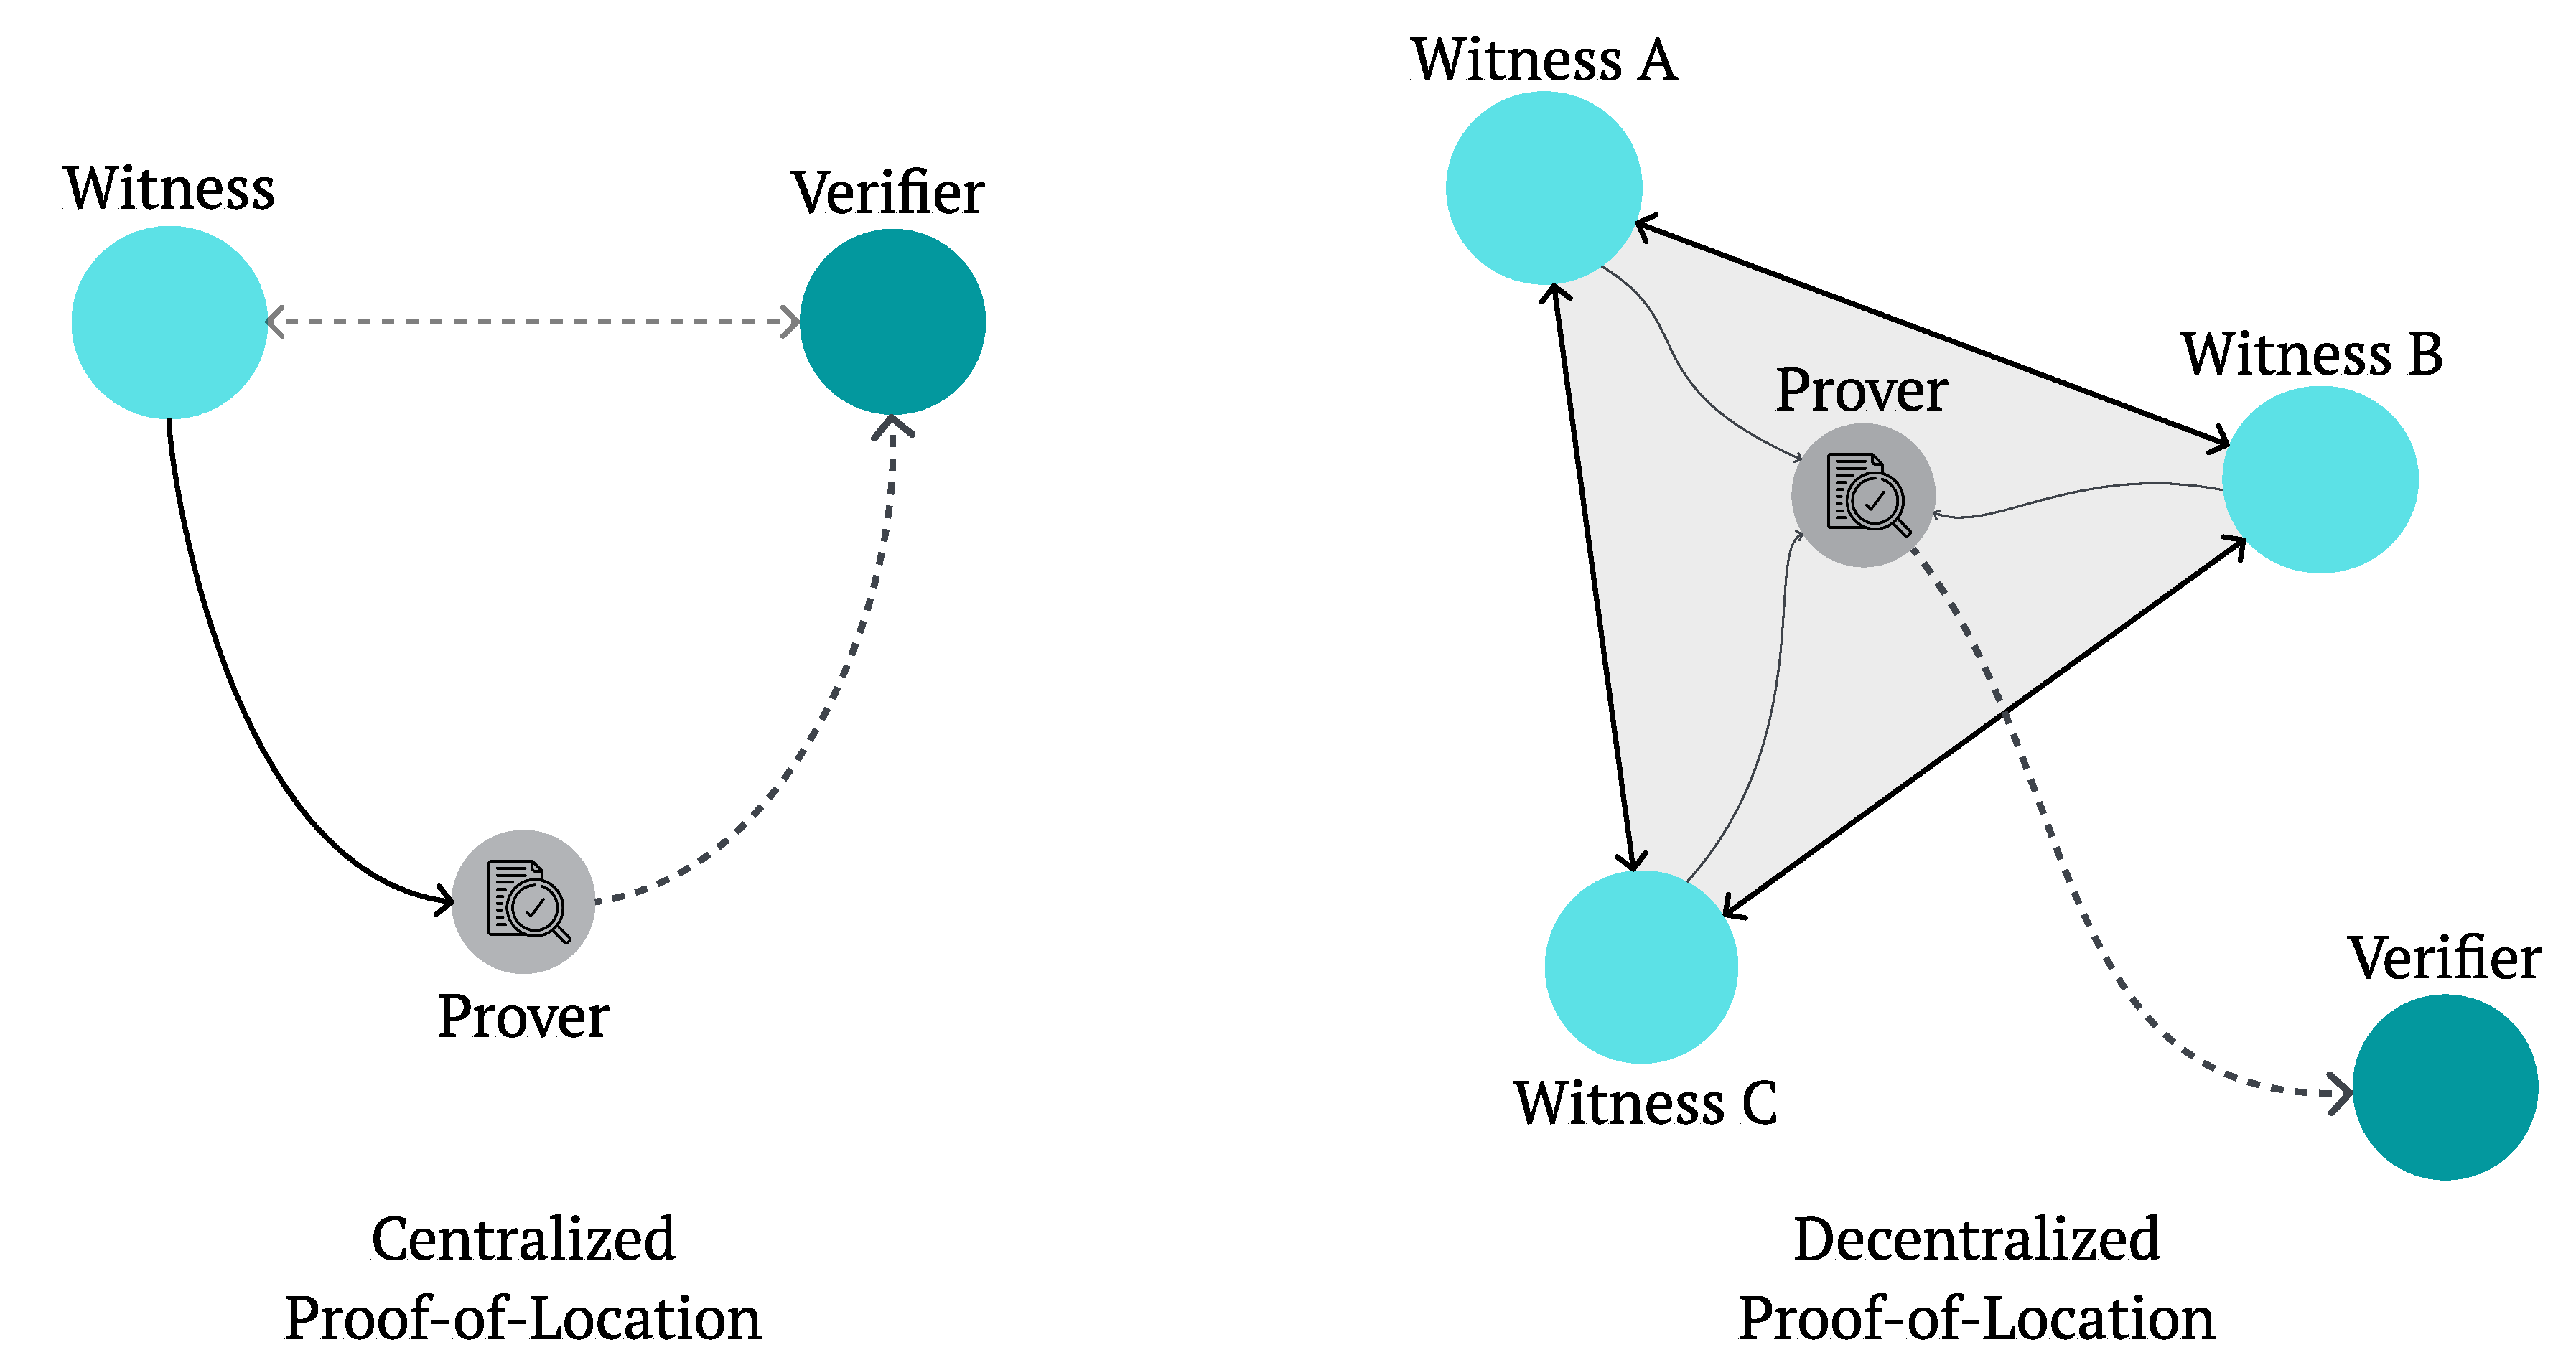
\includegraphics[width=0.9\textwidth]{proof-of-location-protocol-entities.pdf}
    \caption{The entities involved in a \pol{} protocol. The left side of the figure represents the typical arrangements of a centralized protocol, where the witness and the verifier may establish some bond between each other. The right side shows the configuration of a decentralized and trustless solution, where a quorum of witnesses attests the prover's location.}
    \label{fig:proof-of-location-protocol-entities}
    \end{center}
\end{figure}

\paragraph{Prover.} A prover is a dynamic entity, both in movement and availability terms. It is expected to be able to communicate with the witnesses, to gather a proof of its location, and to be later able to provide a location claim to the verifier. Communication with nearby witnesses is thought to happen via any short-range message transmission means. Provers are also expected to be associated with a verifiable but desirably private identity, often as a pseudonym.

\paragraph{Witness.} A witness is an entity that is expected to be able to communicate with the prover via the same short-range communication channel and to provide it with a verifiable piece of location attestation. These parties are envisioned to statically or dynamically exist around the prover's location, during the protocol process, and to maintain, in the most recent decentralized protocols, a relatively stable neighbouring list of nearby peers. Witnesses are also expected to be fictitiously identified, usually by a pseudonym.

\paragraph{Verifier.} A verifier is an external entity that is able to receive a location claim from a prover and verify its validity. Although possible and predicted for trusted setups, in a trustless environment and with the general assurances of a permissionless protocol, verifiers shall not have the need to communicate directly with the witnesses. Verifiers' identity is also of no specific importance for the protocol, since the interaction with the prover is usually asynchronous and external to the witnessing process. \\

% Chapter~\ref{sec:related-work} will describe these possible configurations in greater detail, discriminating both their infrastructural layouts and their trust assumptions.

Inspired by \cite{nasrulin2018robust, dupin2018location}, we now introduce a substantially formal but general definition of the \pol{} problem, along with some of its desirable properties:

\paragraph{Definition 1 (\pol{}).} A \pol{} is a verifiable digital certificate that attests the presence of a prover $\rho$ at location $l$ and time $t$.

\paragraph{Definition 2 (Completeness).} A \pol{} is complete if the prover $\rho$ is attested at location $l$ and time $t$, by a set of witnesses $\omega \in W$.

\paragraph{Definition 3 (Spatio-temporal Soundness).} A \pol{} is spatio-temporally sound if it is generally hard for the prover $\rho$ to obtain, forge, or modify a complete \pol{}, if not physically present at location $l$ and time $t$.

\paragraph{Definition 4 (Non-transferability).} A \pol{} is non-transferable if valid only for the prover $\rho$ that obtained it.

\paragraph{Definition 5 (Correctness).} A complete \pol{}, generated by an honest prover $\rho$, in cooperation with honest witnesses $\omega \in W$, must always be accepted by an honest verifier $\nu$.\\

Additional properties may be protocol specific, but the above definitions are generally considered to be the most common and desirable properties of a \pol{} protocol. Further formalizations can be found in the works dissected in Chapter~\ref{sec:related-work}.

\subsubsection{Common Threat Models}

Like with any technology that involves the collection and processing of sensitive and tamper-prone location data, \pol{} systems must be designed and implemented with a keen awareness of the threat landscape. The threat models of these systems are very often intricately multisided, encompassing a diverse range of actors, motives, and attack vectors. In this context, it is crucial to understand not only the technical mechanisms of \pol{} systems, but also the broader factors that shape their security and privacy risks. 

Some common scenarios that may affect the security of \pol{} systems are, for instance, malicious provers that may attempt to forge location claims, or witnesses that may attempt to collude with other entities to falsify the information. Adversary efforts may also be observed in the form of baleful provers, or witnesses, that may try to respectively impersonate other peers. Sybil attacks are too on the horizon of possible threats, often employed to disrupt the operation of the system by flooding it with fake participants \cite{nasrulin2018robust}. Other works have also considered semi-honest adversaries that, despite following the protocol rules, may try to learn additional information from the messages exchanged \cite{dupin2018location}. These and other attack vectors are further dissected in Chapter~\ref{sec:related-work}, with reference to the multiple solutions that attempt at being shielded from these malicious situations.

\subsubsection{Application Scenarios}
\label{sec:background-proof-of-location-application-scenarios}

The concept of verifiable and digital \pol{} has a wide range of applications, as deconstructed by Sariou and Alec, in \cite{saroiu2009enabling}. For instance, in customer reward systems, \pol{} can be used to provide incentives to customers who visit physical stores, offering rewards and loyalty programs to verified visitors. In location-authenticated business review systems, \pol{} can be used to verify the authenticity of customer reviews. By requiring customers to verify their physical presence at the business location, businesses can prevent fake reviews and ensure that only genuine customer feedback is posted. In location-restricted web content delivery, \pol{} can be used to limit access to online content based on the user's physical location. For example, a video streaming service may use verifiable \pol{} to prevent users from accessing content outside legally allowed regions or countries. In voter's physical presence verification, a \pol{} protocol can be set to prevent voter fraud, by verifying that voters are physically present at the polling stations. Remote working and residency verification, for tax purposes, fit too in the realm of possible applications. Pournaras \cite{pournaras2020proof} goes beyond these specific cases and theorizes about an augmented democracy approach to smart city development. In the author's hypothesis, \pol{} is used to create a transparent and participatory decision-making process by enabling citizens to verify their physical presence at public meetings and events. \pol{} may also play a role in the smart mobility infrastructure, helping in verifying and optimizing the use and cost of public transportation.

Tailored to the reality that wraps the writing of this thesis, this problem becomes increasingly relevant with the advent of Artificial Intelligence (AI) tools, capable of forging highly realistic content at unprecedented scales. To combat such surge, photographers, and reporters may make use of \pol{} to certify the physical originality of their photos and videos, while journalists may use it to verify the authenticity of their sources. Another use case is the verification of the provision of services, such as the delivery or supply of goods, by third-party providers. For instance, an Internet Service Provider (ISP) may use \pol{} to attest the physical deployment and provision of connectivity to a group of customers in a particular area. This can be extended to attest, as well, the quality of the service and to prevent the ISP from charging for services that are not provided, increasing overall trust and transparency. For the first use case, let's imagine a reporter who arrives at an accident site, in a busy city centre. The reporter takes out his camera and captures photos and videos of the crash. As he records, several bystanders notice and approach him. As they all simultaneously witness the reporter's presence at the accident site, they are able to attest his physical presence at the location and time of the event, certifying the authenticity of the content that would feature later in the news. In the second use case, there is a group of customers that have been waiting for a long time for their ISP to provide connectivity to their neighbourhood. The ISP has been charging them for the service, but the customers have not been able to use it. The ISP, however, has been claiming that the service is being provided, and that the customers are not entitled to a refund. The customers, then, decide to coordinate their efforts and to attest the ISP's service provision in their neighbourhood. They all synchronously connect their devices to the infrastructure and attest the ISP's connectivity, proving it is not providing the expected service. They proceed to sign the attestation and file a complaint to the regulatory authorities. These two examples are depicted in Figure~\ref{fig:proof-of-location-example-scenarios} and will feature in the following chapters, bridging the specification of the \pol{} protocol with real world use cases.

\begin{figure}[h!]
    \begin{center}
    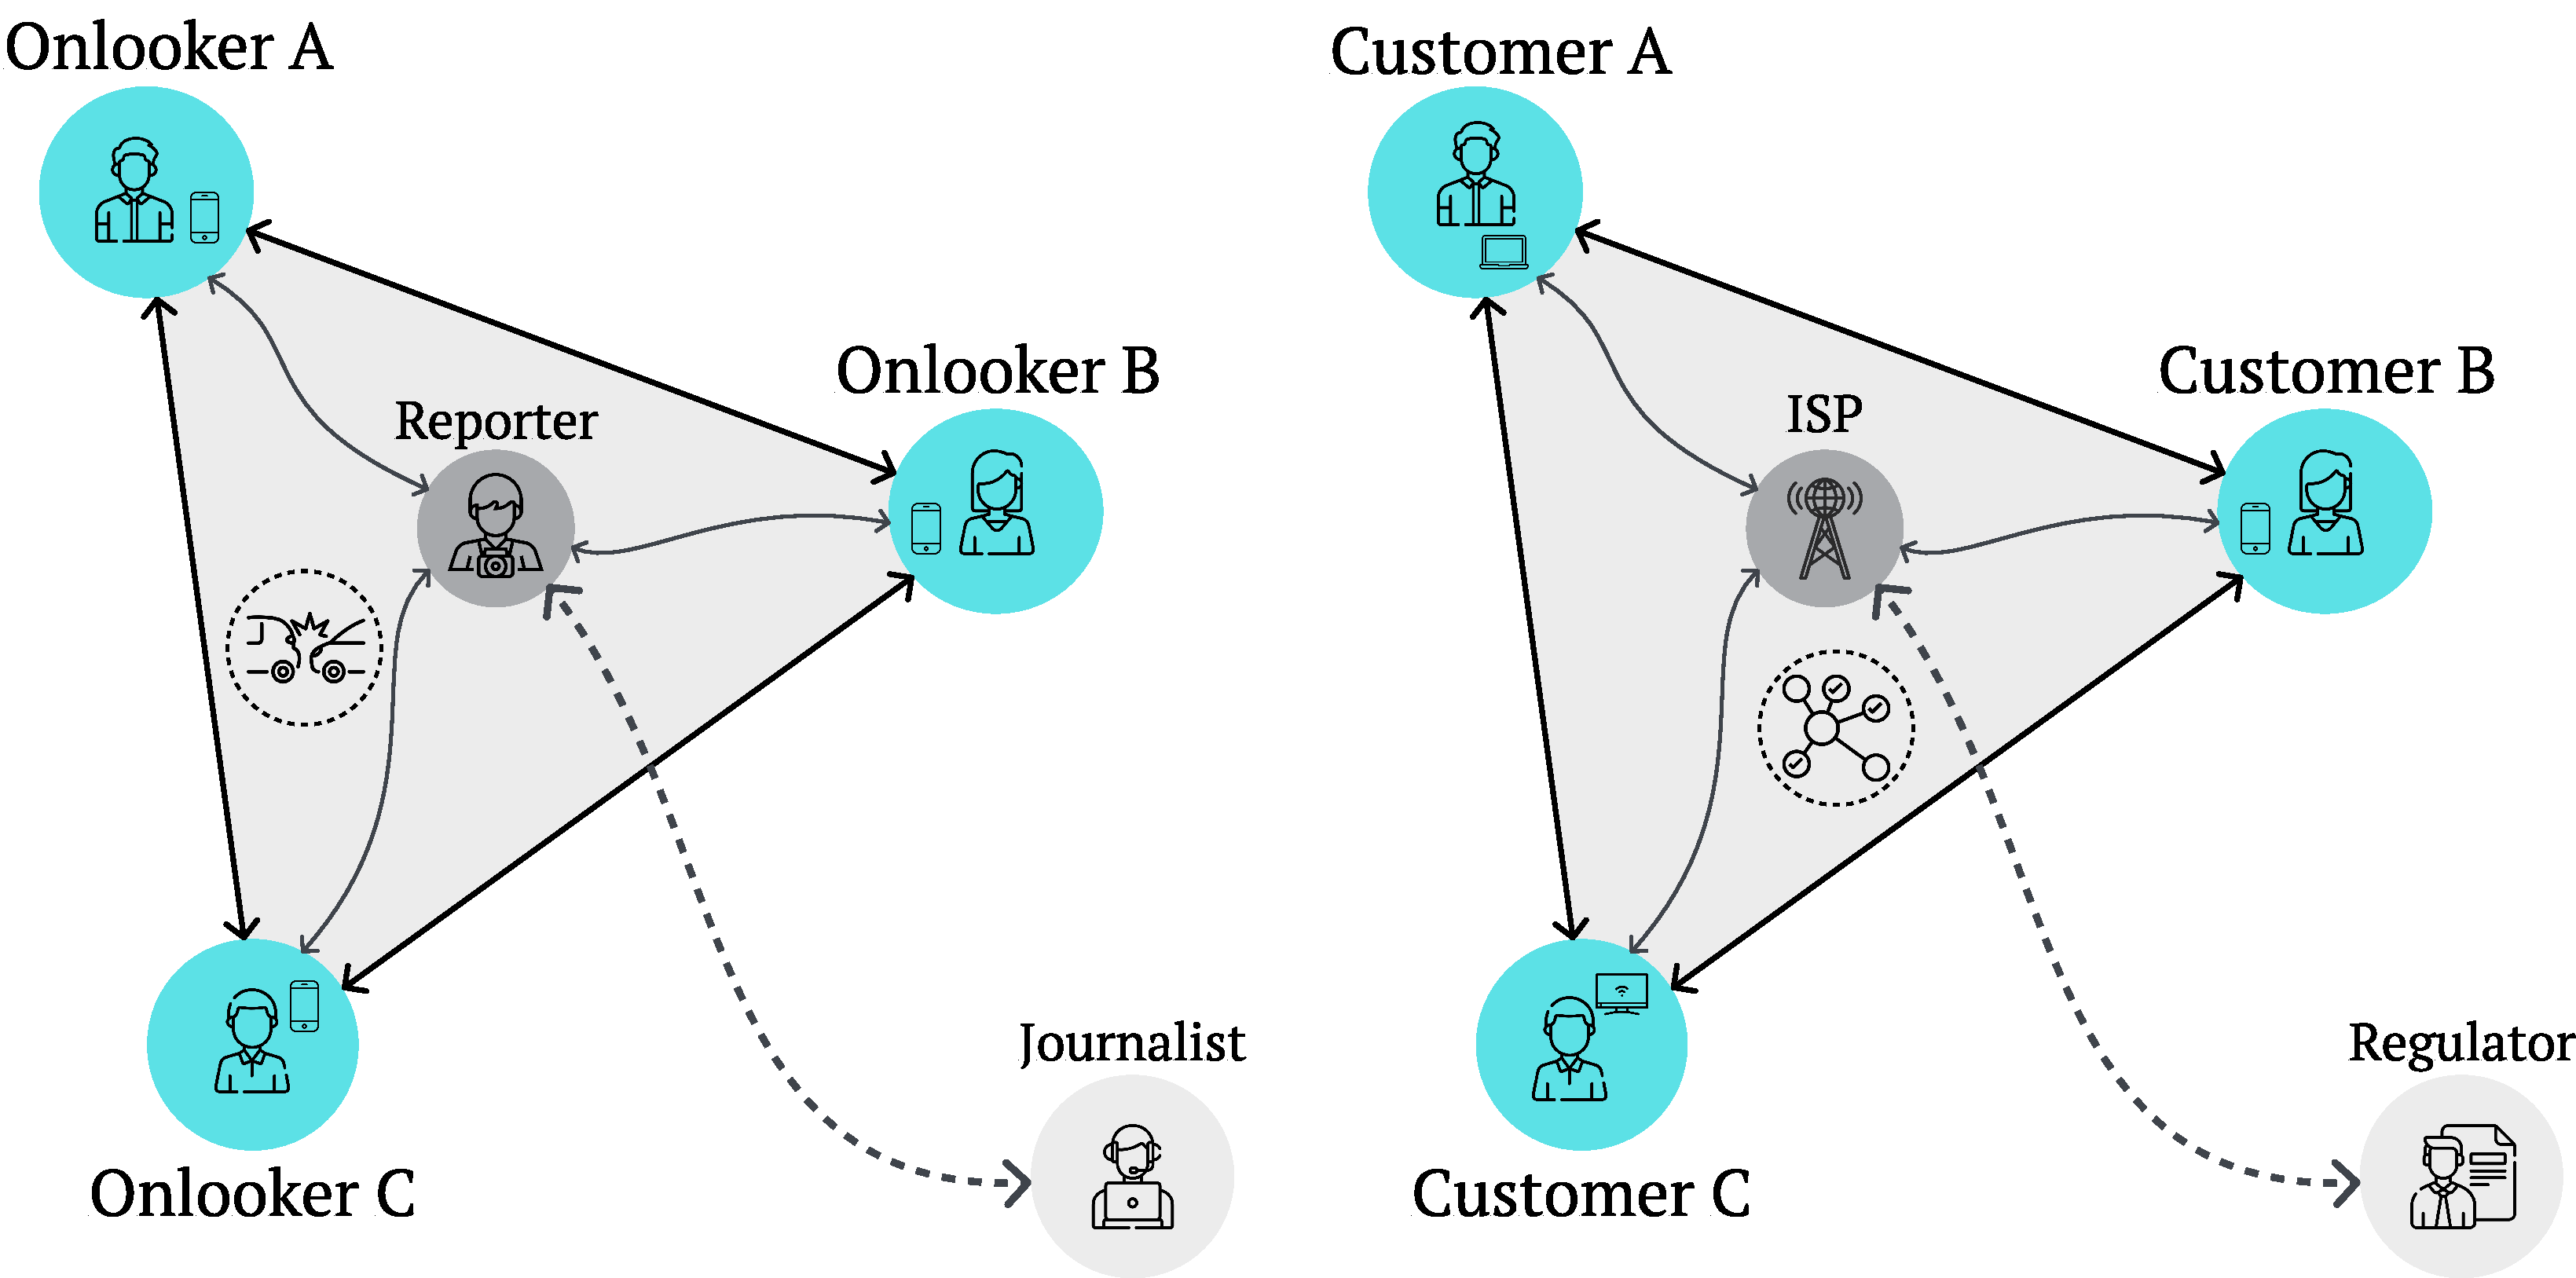
\includegraphics[width=0.9\textwidth]{pol-examples.pdf}
    \caption{Examples of \pol{} applications.}
    \label{fig:proof-of-location-example-scenarios}
    \end{center}
\end{figure}

Targeting different trust levels, additional application scenarios can be derived from the above, while many others are yet to be discovered. Given all this, digital and verifiable \pol{} has a wide range of applications that may disruptively benefit individuals, businesses, and the society as a whole. Chapter~\ref{sec:related-work}, afterwards, gives a more nuanced overview of both the evolution of the protocols and specific use cases that these multiple solutions aim at covering. The next section will introduce the technologies that are set to enable short-range communication between the entities of a \pol{} protocol.

\subsection{Wireless Mesh Networks}

Dynamic and non-hierarchic mesh networks are a type of wireless network architecture that allows for the creation of ad hoc networks in which nodes can communicate with each other without the need for a central coordinating device. This type of network is characterized by its ability to self-organize and dynamically adapt to both changes in the environment and in the overall network topology. As presented in Section~\ref{sec:background-wireless-mesh-networks}, one of the key features that materializes the concept of dynamic and non-hierarchic mesh networks is the existence and implementation of lower-layer routing protocols to facilitate the peer-to-peer communication between the nodes.

Mesh networks, as expected, rely first on the physical layer, according to the standards of computer networking, which is responsible for transmitting raw bit stream data over the physical medium, copper wire, optical fibre, or wireless frequencies, for example. This layer defines the physical characteristics of the data transmission, such as voltage levels, data rates, and the physical connectors and media used for communication. Its main function is to provide a reliable and efficient transmission of bits between devices, without any regard made to the higher-layer protocols and their associated data. The physical layer is responsible for encoding and decoding data into a format that can be transmitted over the network, while also detecting and correcting errors that occur during transmission \cite{peterson2007computer}. It also defines the substrate physical topology of the network, which describes the arrangement of the physical components such as devices, cables, and other network equipment, as depicted in Figure~\ref{fig:proof-of-location-overview-pol-mesh}. To then enable efficient and coordinated communication, there is a need for routing protocols that determine the best path for data packets to travel through.

\begin{figure}[h!]
    \begin{center}
    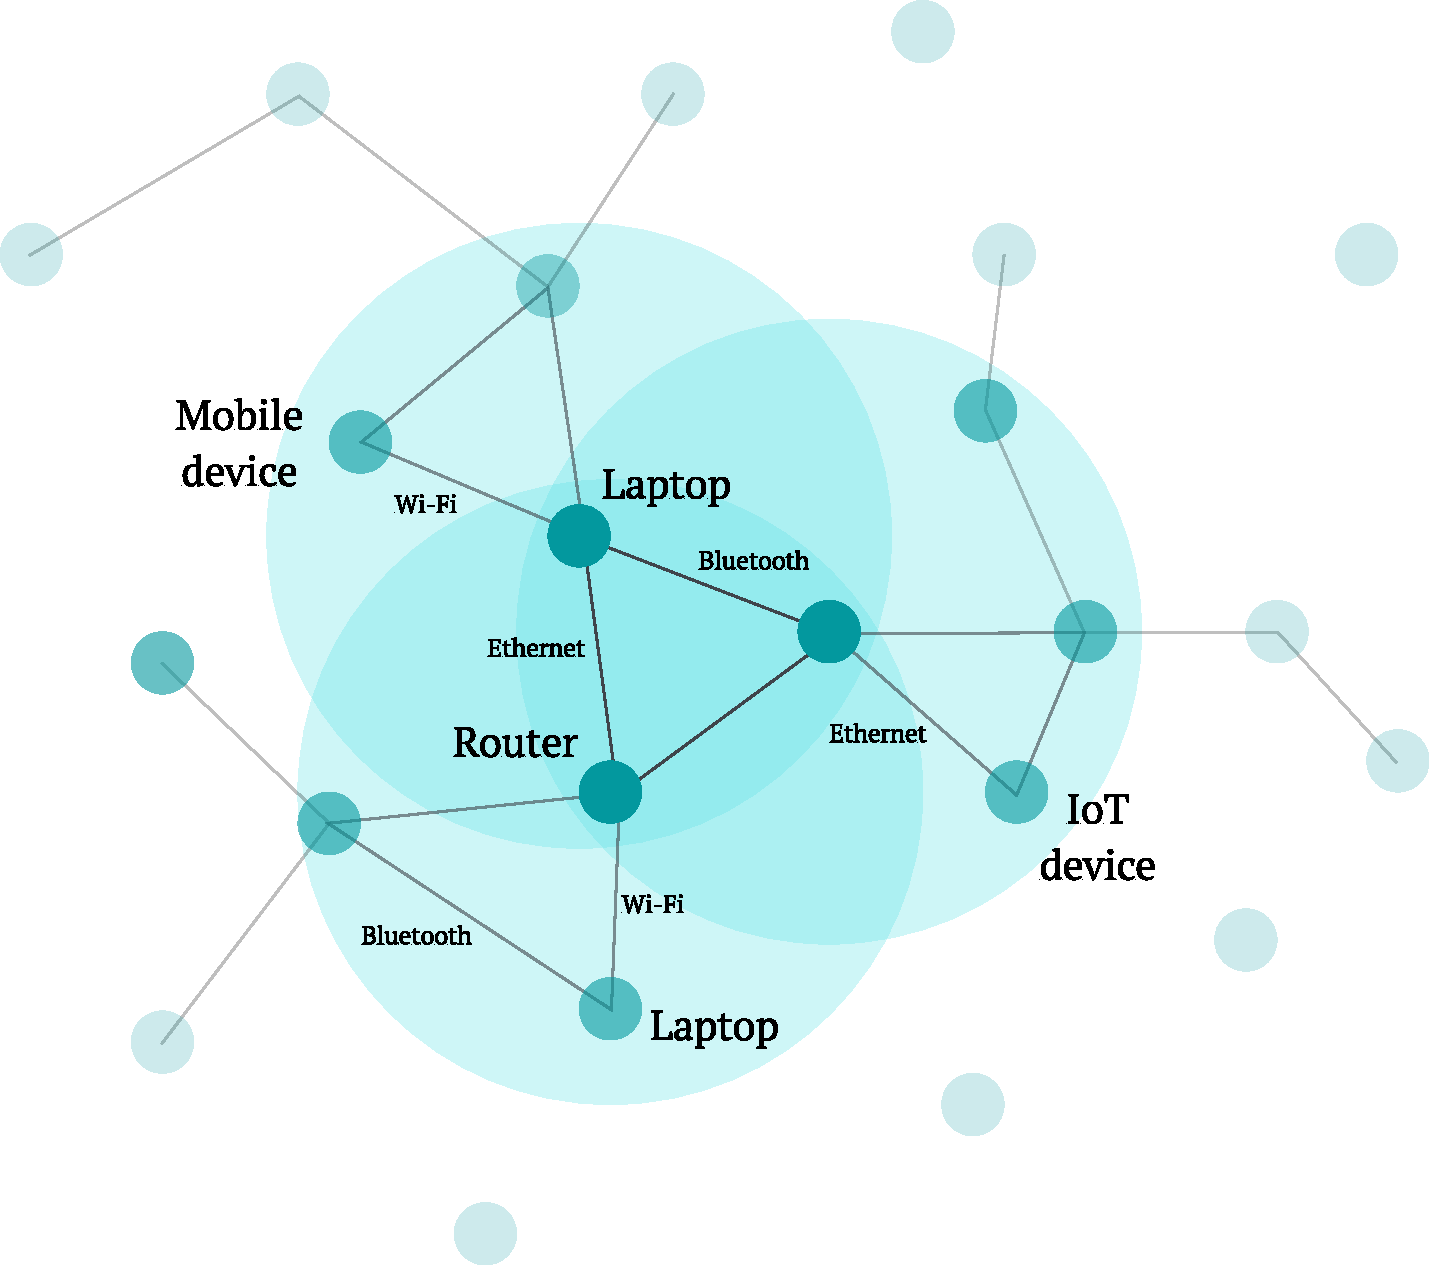
\includegraphics[width=0.65\textwidth]{overview-pol-mesh.pdf}
    \caption{The heterogeneity of a Mesh Network and the substrate diversity of its physical topology~\textemdash~the devices, their connections, and their physical arrangements.}
    \label{fig:proof-of-location-overview-pol-mesh}
    \end{center}
\end{figure}

These routing protocols are expected to operate, not at the network layer, but instead at the data link layer, which is responsible for handling the transmission of data frames over the physical layer. Their main goal is to determine the best path for data frames to travel, based on metrics gathered from lower-level physical information, as, for instance, signal strength and link stability metrics \cite{misra2009guide}. These protocols can support neighbourhood discovery and the ranking of neighbours \cite{batman-adv-v}, and thus potentially enable the processes of zone establishment and zone affinity management, as illustrated in Figure~\ref{fig:proof-of-location-overview-pol-zone-establishment}. Neighbourhood discovery is the process of physically discovering neighbouring nodes within the mesh network \cite{open-mesh-ogmv2}. Neighbour ranking is the process of determining the quality and reliability of each neighbouring link \cite{seither2011routing}. By measuring, understanding, and ranking the quality and reliability of the data links, and by instructing nodes to independently calculate their best next-hops, a routing protocol can establish neighbourhoods and determine the affinity of nodes within these coverage localities. This information can be primarily used to optimize communication paths, reduce congestion, and increase the overall efficiency of the network.

\begin{figure}[h!]
    \begin{center}
    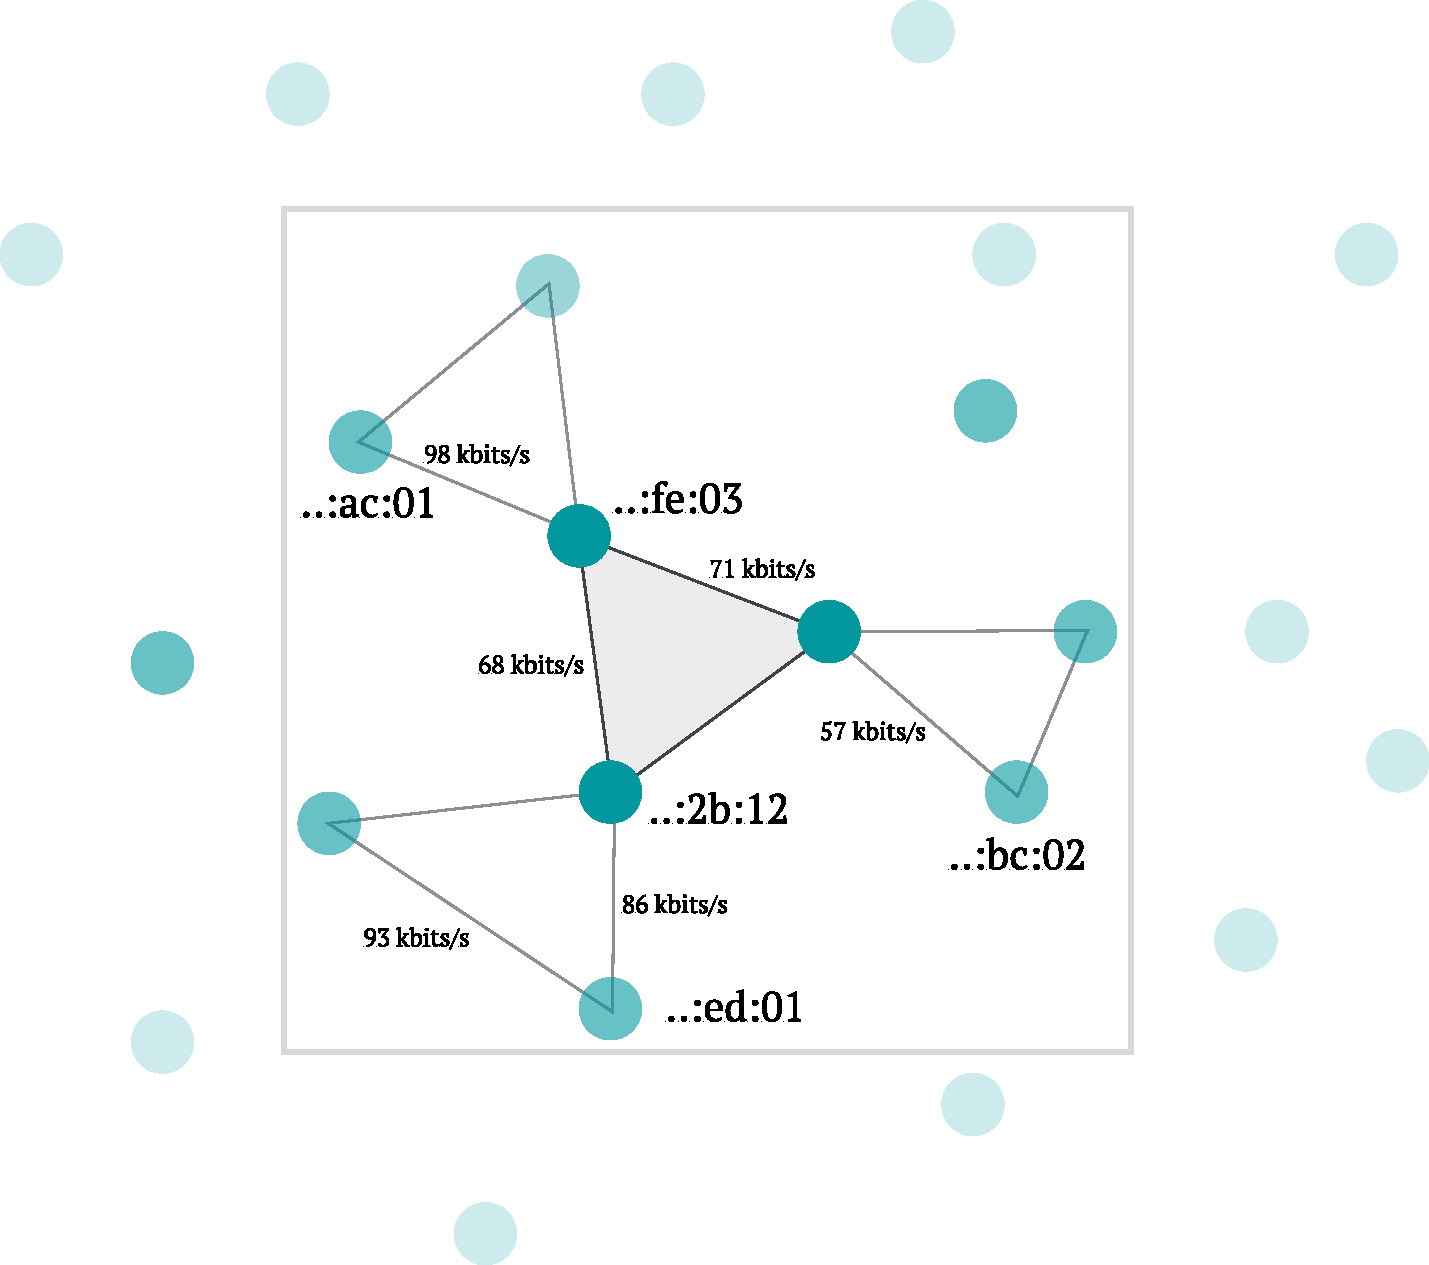
\includegraphics[width=0.7\textwidth]{overview-pol-zone-establishment.pdf}
    \caption{The routing protocol's neighbourhood discovery and ranking processes, using the MAC sublayer and link quality metrics, to enable the establishment of zones within the mesh network.}
    \label{fig:proof-of-location-overview-pol-zone-establishment}
    \end{center}
\end{figure}

The second usage of such accomplishment is to finally enable the targetted establishment of zones within the mesh network. Zones can be viewed as strongly connected sets of neighbours, that, in consequence, are one-hop away from each other. This process of zone establishment is facilitated by the routing protocol, but not strictly enforced, as the protocol solely enables the discovery of potential neighbours and the ranking of their links. The final decision of which nodes are to be grouped together into a zone is left to the nodes themselves, which can then use this information to establish their own zone affinity. Zone affinity is the process of determining the likelihood of nodes communicating and establishing zones with other nodes. The motivation may also be extrinsic to the process of zone discovery or establishment. An identity management protocol, for instance, can be used to determine the zone affinity of nodes, based on their identity and their individual wishes to communicate with other nodes. Incentives of higher degree can be used to motivate nodes to communicate, to establish zones with other relatively specific sets of nodes, and hence to collaborate in the next step of providing zone-relative location services. 
\TODO{Above is too abstract, need example...}
The FOAM protocol, for example, envisions the reliance on token-curated registries to provide a decentralized identity management. It may also rely on crypto-economic incentives to motivate nodes to collaborate and, together, establish and maintain coverage zones, for the higher purpose of providing \pol{} capabilities \cite{foam-white-paper}. This thesis' main focus, with regard to the \poc{} implementation, is abstracted from the whole process of zone establishment and zone affinity management, and assumes that a zone has been already agreed to be established by some out-of-band process. Nonetheless, these aspects are still to be identified for future work, as they are essential for the overall success of the protocol.

After the establishment of operational zones and the affinity filtering potentially happening at the data link layer, the typical Internet Protocol or TCP/IP suite can be used to enable end-to-end data communication for application-specific purposes. The TCP/IP suite consists of a set of protocols that operate at the network and transport layers, providing end-to-end communication services for applications running on different nodes \cite{peterson2007computer}. At the network layer, the Internet Protocol (IP) is used to route data packets within and between the zones, based on their IP addresses. IP is a connectionless protocol that operates independently of the underlying physical and data link layers, allowing it to be used with a variety of network technologies. At the transport layer, protocols such as TCP and UDP can be used to enable end-to-end data communication between application instances. TCP is a reliable, connection-oriented protocol that provides features such as flow control, error detection, and congestion avoidance to ensure that data is transmitted reliably and efficiently between applications. UDP, on the other hand, is a connectionless protocol that provides a lightweight alternative to TCP, suitable for applications that require low-latency communication or do not require reliability guarantees at the transport layer \cite{peterson2007computer}. The choice between the two may be based on the application requirements, the network topology, and the available resources, but the overall conclusion is that, after enabling network layer capabilities, any typical Internet service can be provided to the end-users, sustained by the underlying mesh network. Additionally, as pictured in Figure~\ref{fig:proof-of-location-overview-pol-zone-affinity}, by subnetting and assigning a unique range of IP addresses to each zone, nodes can communicate with each other, in the same zone, and with nodes in other zones using IP-based protocols. Subnetting can also provide a range of benefits, such as improved security, better network management, and more efficient address assignment and usage \cite{peterson2007computer}.

\begin{figure}[h!]
    \begin{center}
    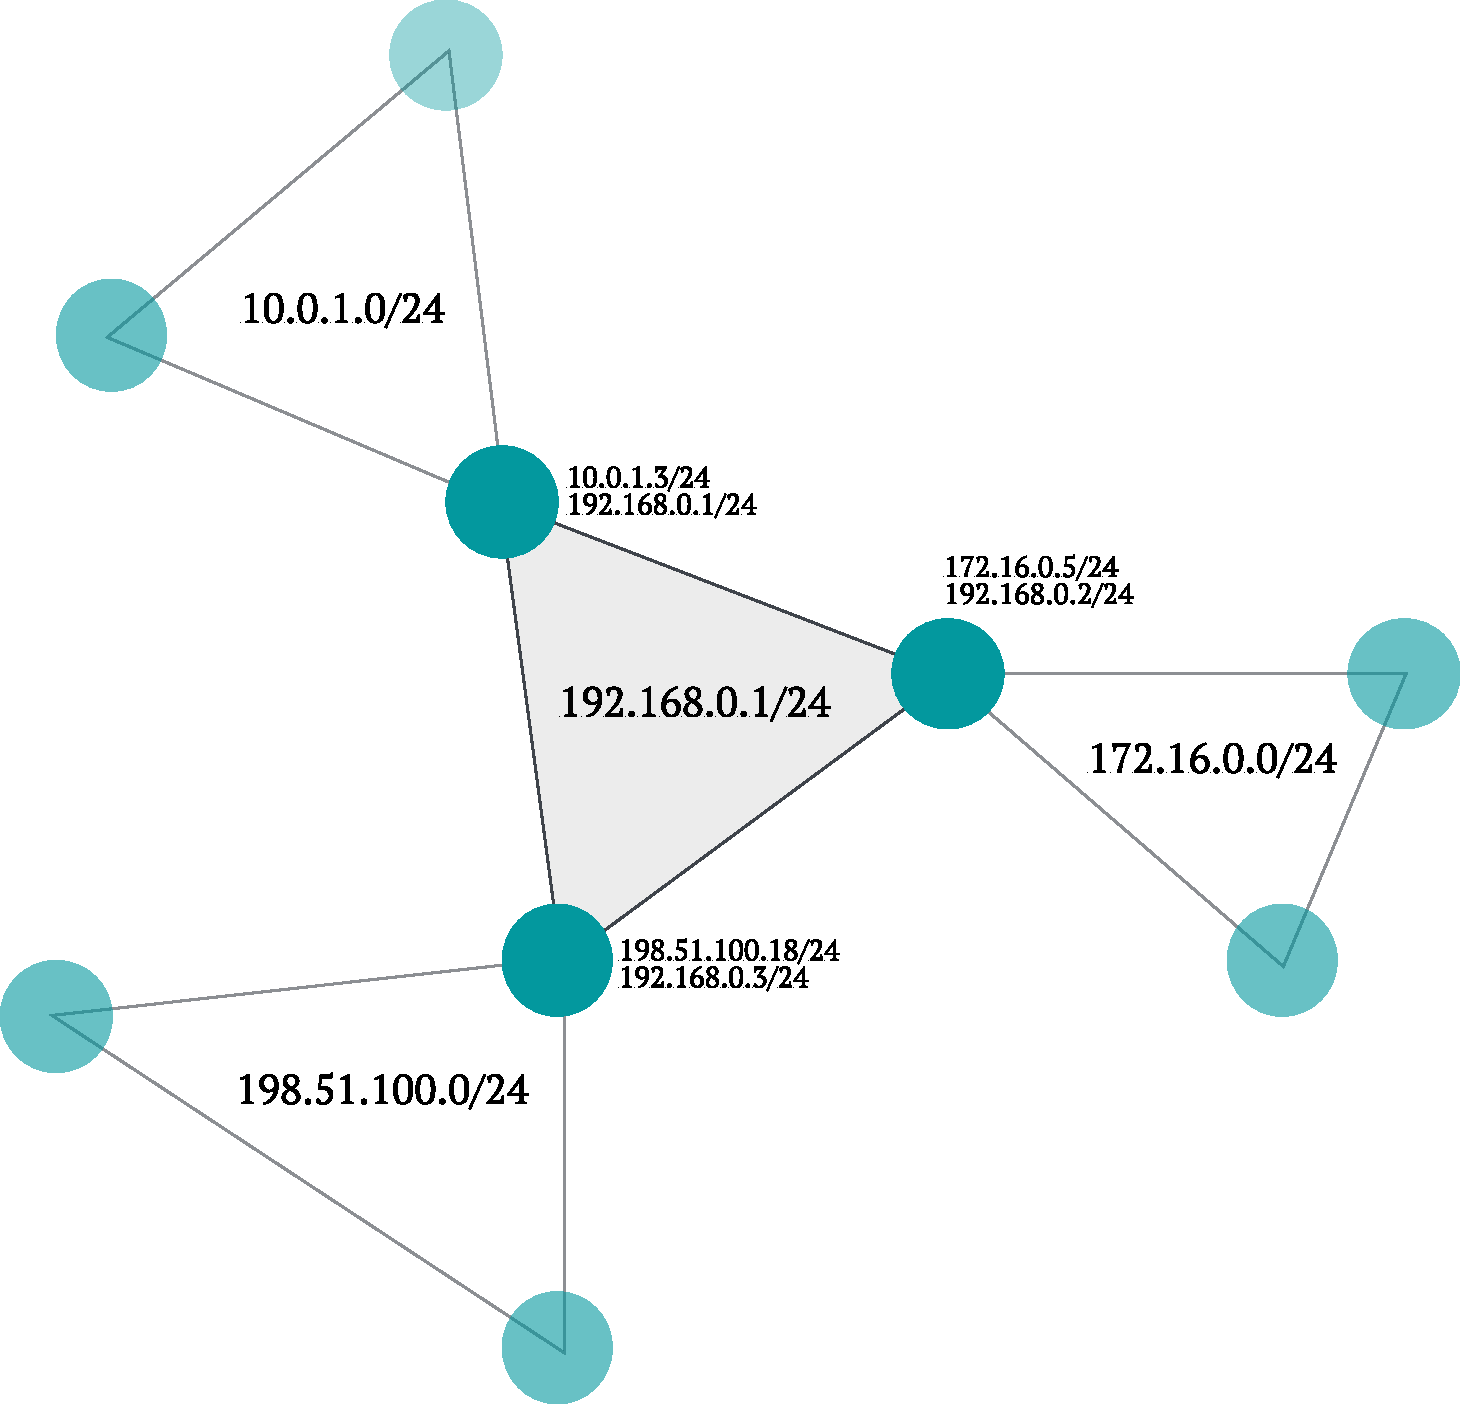
\includegraphics[width=0.6\textwidth]{overview-pol-zone-affinity.pdf}
    \caption{Subnetting and IP-based communication between nodes, within and between zones, after the establishment of their respective zone affinities.}
    \label{fig:proof-of-location-overview-pol-zone-affinity}
    \end{center}
\end{figure}

The following section presents the next step towards guaranteeing the infrastructural basis of the proposed \pol{} protocol, detailing not only the need for zone-relative clock synchronization, but also the steps taken to eventually achieve spatio-temporal soundness. It ultimately assumes that the physical, data link, network, and transport layer capabilities have been already established, and that the nodes are able to communicate with each other using the TCP/IP suite and related protocols, on top of the underlying mesh network infrastructure. The verification or enforcement of the usage of short range communication means is still to be researched, as a key aspect to the protocol's foundational security, and soundness guarantees.

\subsection{Permissionless Consensus}

Long has been the time when consensus was still on the verge of being considered such a fundamental problem of distributed systems. Generally defined by Lamport, et al. \cite{pease1980reaching, lamport2019byzantine}, consensus means reaching an agreement between multiple parties in the potential presence of faulty individuals. As per multi-agent systems, interacting over computer networks, consensus is thought to be the result of a coordination effort, that eventually leads the parties to agree on some value at a given moment. However, the evolution of the consensus problem has been invariably limited by a set of strong assumptions. The well-known Byzantine-Fault-Tolerant multiparty consensus systems, that have been designed over the years, are usually meant to work only with a set of known participants, being them faulty or not \cite{castro1999practical}. 

The other side of the coin is the permissionless consensus challenge, consisting of achieving agreement in an environment where the parties are unknown and untrusted \cite{nakamoto2008bitcoin, buterin2014next}. The relative openness and lack of any kind of central authority are other intrinsic particularities of this type of networks, which inevitably adds complexity to the problem. The participants are not only unknown and untrusted but can also join or leave the network at any time, freely choosing if they care to participate in the consensus protocol. Nevertheless, the problem of permissionless consensus is still seen as a special case of the general consensus definition, but under more meticulous trust assumptions.

Further in this thesis, we will evaluate the different high-level proof-of-location protocols and draw a parallel between the evolution of their trust levels and the ultimate need for a low-level permissionless consensus algorithm that allows for establishing decentralized and time-conscious agreement, in an eventual trustless setup, between the multiple witnesses. The next subsections will briefly review some of the most relevant aspects and proof units that give practicality to the roots of the problem.

\subsubsection{Proof-of-X}

The solution is, nevertheless, unsettled and the scientific community has been reasoning about the need for permissionless consensus when there are already well known and established consensus protocols that work in trusted environments \cite{castro1999practical, miller2016honey}. However, even those protocols have their own limitations, not only in terms of trust, fault-tolerance, centrality, permissions, or bottlenecks, but also in terms of scalability \cite{miller2016honey}, despite assuring deterministic finality \cite{decker2016bitcoin}. The need for permissionless consensus is then justified by the fact that permissioned protocols are not compatible with the requirements of the new generation of distributed systems, especially in the context of Blockchain networks. These requirements include dealing with today's sparse networks of anonymously and dynamically participating devices, without interrupting consensus and while battling Sybil attacks \cite{8629877, survey-dist-consensus}. Fundamentally, the permissionless consensus problem is the need for a consensus protocol that can be run in a distributed and decentralized environment, where the participants are unknown and untrusted, and where the network is bigger, sparser and unpredictably less reliable.

Technically, permissionless environments allow for larger networks that depict lower connectivity between the participants. Operationally, everything is expected to happen in an asynchronous or partially synchronous fashion, and the number of transactions is predicted to be smaller than in the permissioned counterparts. Participation is free, and the governance is not centralized, but rather distributed and public. The identity of the participants is secured or semi-secured as it often relies on pseudonymity for protecting the nodes' identity, enabling, at the same time, full transparency concerning the rest of the network's content and operation \cite{xiao2019distributed}. Expectedly, the goal of permissionless consensus, as for any consensus protocol, is to reach agreement on a single value, or a set of values. However, due to the nature of the protocols, the values that are agreed upon end up establishing the serialization of the transactions, and so establishing time consciousness and total order of the events \cite{8629877}.

\begin{figure}[ht]
  \begin{center}
  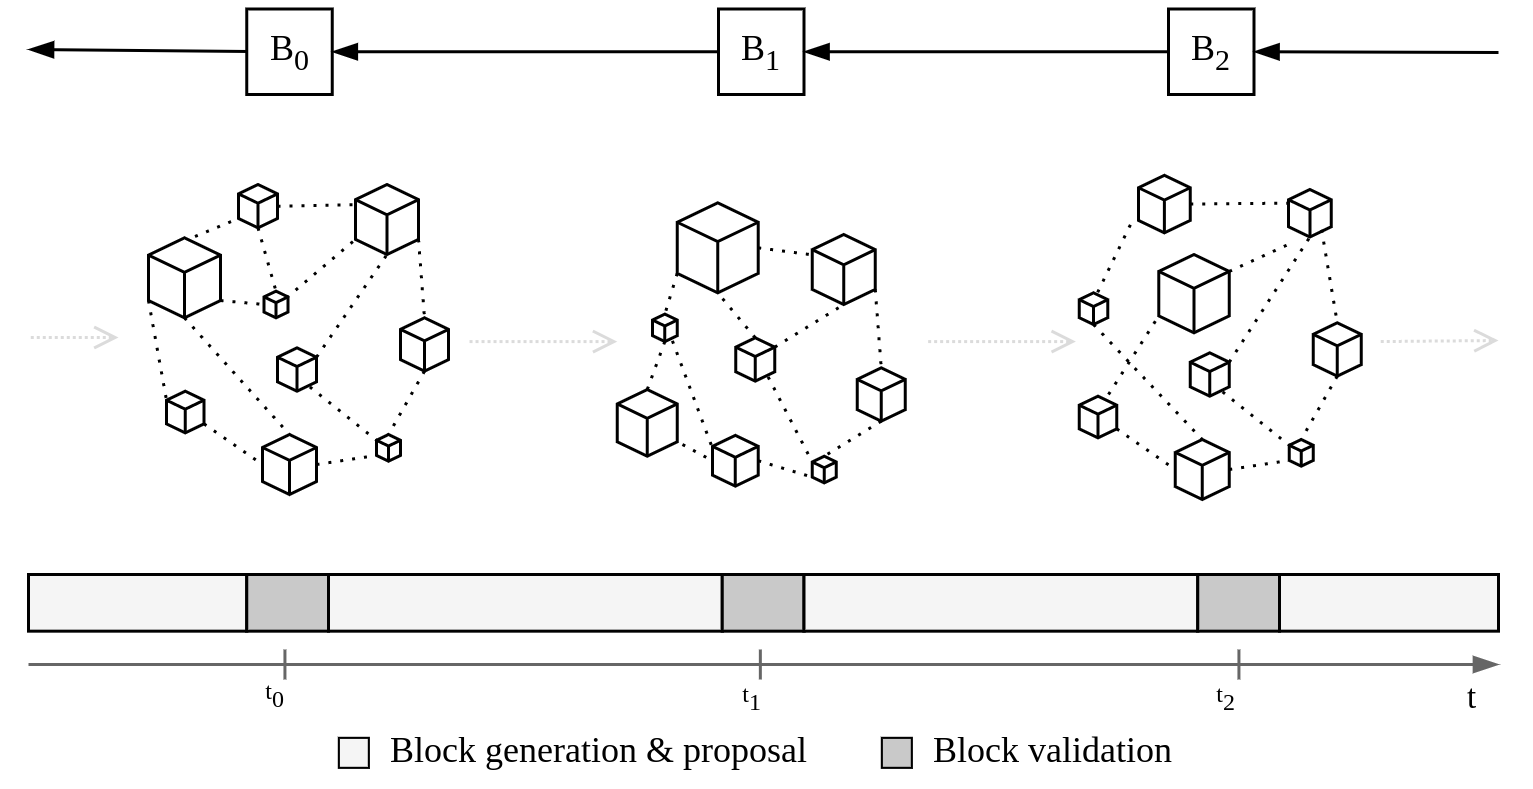
\includegraphics[width=0.9\textwidth]{building-blocks-consensus.png}
  \caption{An illustration of the permissionless consensus building blocks - 
  the block generation and proposal phases followed by the block validation, 
  along with frequent network topology changes and the consequent serialization of the information.}
  \label{fig:building-blocks-consensus}
  \end{center}
\end{figure}

Also described in \cite{survey-dist-consensus}, very concisely, the way to achieve an operating protocol, as seen in the mainstream Blockchain networks, is by first generating the agreeable value, in this particular case, a block and its proof, disseminating the information to the network, followed by the eventual validation and acceptance of the block by the rest of the nodes. This is the approximate moment when consensus is reached (See Fig. \ref{fig:building-blocks-consensus}). During the whole process, a fair and somewhat predictable incentive mechanism is also needed, that rewards participants for their honest effort in reaching consensus, and punishes the ones that are not behaving correctly. These incentives are of major importance in this very context of permissionless consensus and all these building blocks form the basis of the inner functioning of Bitcoin itself \cite{nakamoto2008bitcoin}, replicated with some variations in other permissionless networks \cite{buterin2014next}. The following is a short introduction to some relevant proof units that feature in the most popular Blockchain systems.

\subsubsection{Proof-of-Work and Proof-of-Stake}

Without discrediting the previous attempts, the first practical permissionless consensus algorithm was proposed by Nakamoto in \cite{nakamoto2008bitcoin}. It is a Proof-of-Work consensus protocol that resembles a replicated state machine where the independent participants reach agreement not only about transactional values, but also about their order - naturally forming the underlying structure of what is now known as a Blockchain. The focus shifted for decentralized systems and after Proof-of-Work many other consensus mechanisms have been proposed, relying on different consensus units.

In the classical Nakamoto consensus protocol, the generation of a block, to be proposed for further network agreement, complies with the unit of computational work needed to create, or rather find, a verifiable proof of the effort spent on assembling the block \cite{nakamoto2008bitcoin}. This essentially requires brute forcing the search for a cryptographic hash value for the aggregation of the block information with a nonce. This value has to satisfy a difficulty threshold (See Procedure \ref{proc:BlockGeneration}), which gets adjusted dynamically over time, to maintain the network overall requirement for the block generation interval \cite{8629877, survey-dist-consensus}.

\begin{procedure} [!h]
	\caption{BlockGeneration()} \label{proc:BlockGeneration}
	\KwIn{Transaction Merkel Tree Root, Hash of the last Block, Timestamp, Other.}
	\KwResult{new $Block$.}
	\BlankLine
  $BlockHeader \ \gets$ Transaction Merkle Tree Root
  \\ \qquad $| \ $ Hash of the last Block
  \\ \qquad $| \ $ Timestamp
  \\ \qquad $| \ $ Other\;
  \BlankLine
  \tcp{the preceding zero bits in $target$ depict the mining difficulty}
  \While{$Hash(BlockHeader \ | \ nonce) \geq target$}{
    Increment $nonce$\;
  }
  \tcp{append transactional data}
  \Return new $Block$\;
	%\eIf{error messages were found}{\Return \False\;}{\Return \True\;}
\end{procedure}

One can then exercise the reasoning line and extrapolate the previous block generation mechanism to a \emph{Proof-of-Something} pseudo-random competition in which an entity in possession of a higher amount of a certain resource, either computational power, or stake, or certain currency, or, for instance, a higher amount of storage space, guarantees a higher probability of leading the block generation and proposal, and consequently winning the acceptance by the majority. This is the essence of Proof-of-Stake, as a derivative of the Proof-of-Work mechanism. Here, stake is a traceable and verifiable amount of a certain unit, token or currency, that is owned by a certain entity who wishes to participate in the consensus protocol. The stake works as a form of collateral that is used to guarantee everyone's honesty, in an attempt to reduce the Sybil attack likelihood. And, respectively as in Proof-of-Work with computational power, the higher the stake, the higher the probability of leading the block generation and proposal.

Idealized and inspired by Proof-of-Stake, extending or adapting Proof-of-Work became a popular trend in the Blockchain community. The main idea is to replace the computational power with some other resource, that is more scarce, or more valuable, or more verifiable, or more traceable, to combine multiple resources, or even to add extra requirements to pure Proof-of-Work \cite{survey-dist-consensus}. Not that every one of the options has a considerable potential for entirely solving the permissionless consensus problem, but each one of them may tackle different use cases where consensus needs to be reached, and where different resources are available to make the agreement happen \cite{BOURAGA2021114384, 9376868}. Nonetheless, the design of these consensus mechanisms shall aim for a protocolar choice between a set of properties that form a trilemma: Security, Scalability, and Decentralization. Briefly put, relaxing the security requirements may allow for more scalability, both of which, consequently, have hands tied with decentralization. These trade-offs are of practical consideration when defining the network goals and use cases \cite{survey-dist-consensus}. Further dissection of various classes of Proof-of-Stake based protocols, diverging alternatives to the classic Nakamoto consensus, and comparisons between them can be found in \cite{8629877, survey-dist-consensus, BOURAGA2021114384, 9376868, natoli2019deconstructing}.

With all of the above in mind, we will proceed to review some of the proposed proof-of-location solutions, discriminated by trust levels. Aiming at achieving spatiotemporal agreement among the witnesses, we will reason about the applicability of one of these lower-level permissionless consensus protocol, in the context of a fully decentralized and trustless environment.

% \subsection{How to use references} \label{sec:using_ref}

% \paragraph{Cross-references to figures, tables and other document elements.}
% LaTeX  internally numbers all kind of objects that have sequence numbers:
% \begin{itemize}
% \item chapters, sections, subsections;
% \item figures, tables, algorithms;
% \item equations, equation arrays.
% \end{itemize}
% To reference them automatically, you have to generate a label using \texttt{$\backslash$label\{some-name\}} just after the object that has the number inside. Usually, labels of different objects are split into different namespaces by adding dedicated prefix, such as \texttt{sec:}, \texttt{fig:}. To use the corresponding reference, you must use command \texttt{$\backslash$ref} or \texttt{$\backslash$eqref}. For instance, we can reference this subsection by calling Section~\ref{sec:using_ref}. Note that there should be a nonbreakable space \texttt{\~} between the name of the object and the reference so that they would not appear on different lines (does not work in Estonian).          



% \paragraph{Citations.}
% Usually, you also want to reference articles, webpages, tools or programs or books. For that you should use citations and references. The system is similar to the cross-referencing system in LaTeX. For each reference you must assign a unique label. Again, there are many naming schemes for labels. However, as you have a short document anything works. To reference to a particular source you must use \texttt{$\backslash$cite\{label\}} or \texttt{$\backslash$cite[page]\{label\}}. 

% References themselves can be part of a LaTeX source file. For that you need to define a bibliography section. However, this approach is really uncommon. It is much more easier to use BibTeX to synthesise the right reference form for you. For that you must use two commands in the LaTeX source
% \begin{itemize}
% \item $\backslash$bibliographystyle\{alpha\} or $\backslash$bibliographystyle\{plain\}
% \item $\backslash$bibliography\{file-name\}
% \end{itemize}
% The first command determines whether the references are numbered by letter-number combinations or by cryptic numbers. It is more common to use \texttt{alpha} style. The second command determines the file containing the bibliographic entries. The file should end with \texttt{bib} extension. Each reference there is in specific form. The simplest way to avoid all technicalities is to use graphical frontend  Jabref (\url{http://jabref.sourceforge.net/}) to manage references. Another alternative is to use DBLP database of references and copy BibTeX entries directly form there.   
    
   
% The following paragraph shows how references can be used. Game-based proving is a way to analyse security of a cryptographic protocol~\cite{GameB_1, GameB_2}. There are automatic provers, such as {CertiCrypt\-}~\cite{certicrypt} and ProVerif~\cite{proVerif}.



% \newpage
% \section{How to add figures and pictures to your thesis}


% Here are a few examples of how to add figures or pictures to your thesis (see Figures~\ref{fig:fnCompModel}, \ref{fig:game-based_proofs}, \ref{fig:proveit_screenshot}).

% Rule: All the figures, tables and extras in the thesis have to be referred to somewhere in the text.


% \begin{figure} [ht] %try to place the figure here (next option top of the page) 
% \begin{center}
% 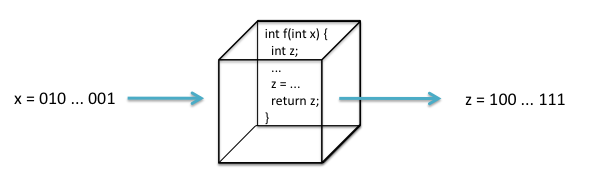
\includegraphics[width=0.8\textwidth]{computational_model_function}
% \caption{The title of the Figure.}
% \label{fig:fnCompModel}
% \end{center}
% \end{figure}



% \begin{figure} [!ht] %if [h] doesn't work, we can force with !
% \begin{center}
% 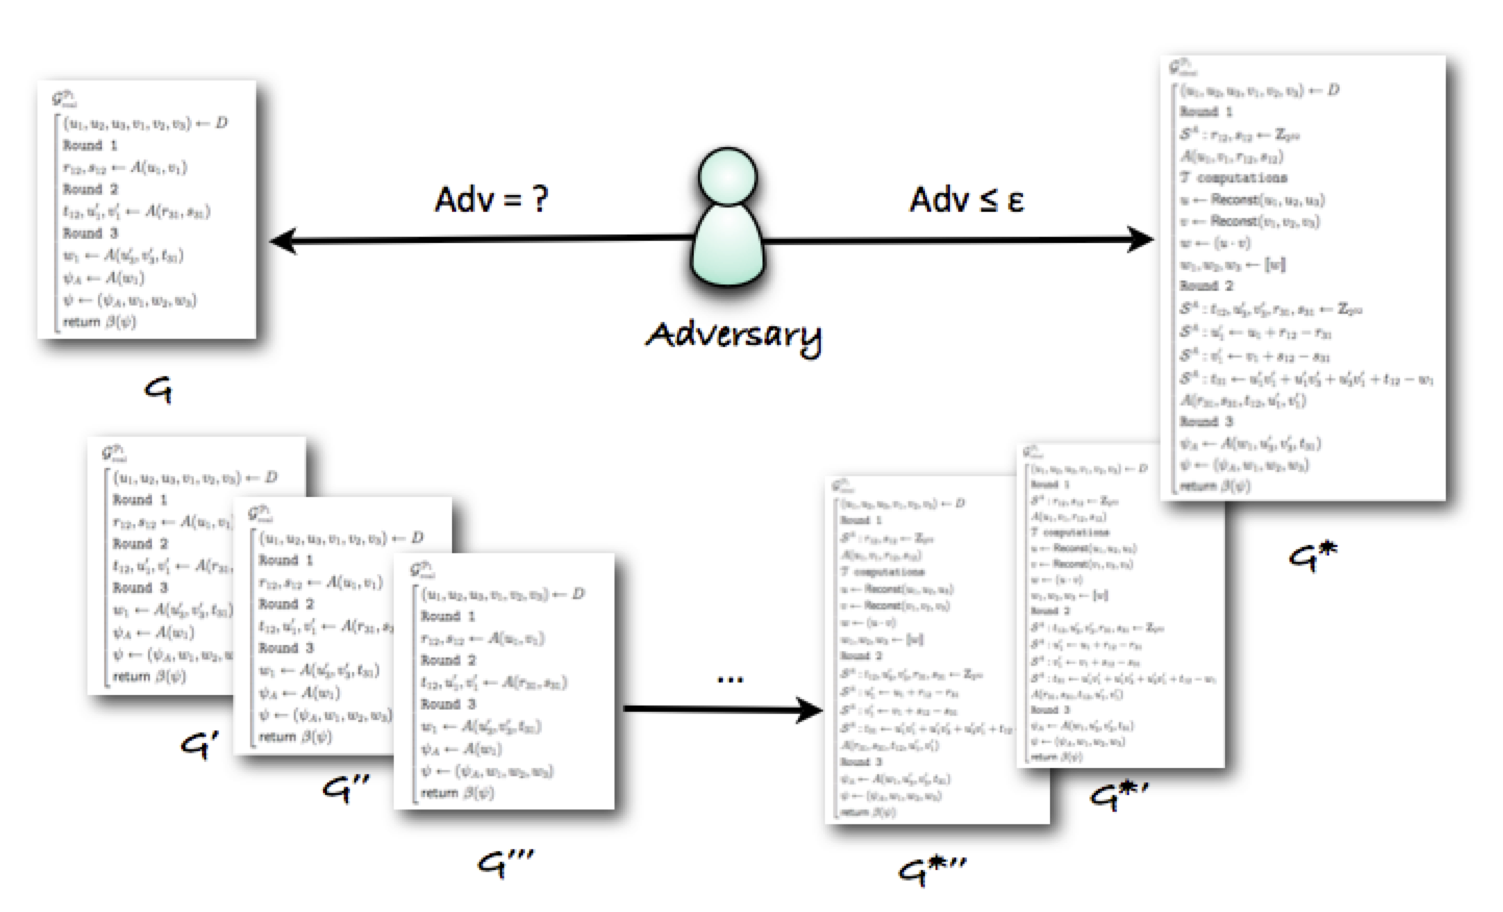
\includegraphics[width=\textwidth]{game-based_proofs}
% \caption{Refer if the figure is not yours~\cite{kamm12}.}
% \label{fig:game-based_proofs}
% \end{center}
% \end{figure}


% \begin{figure} [p]
% \begin{center}
% 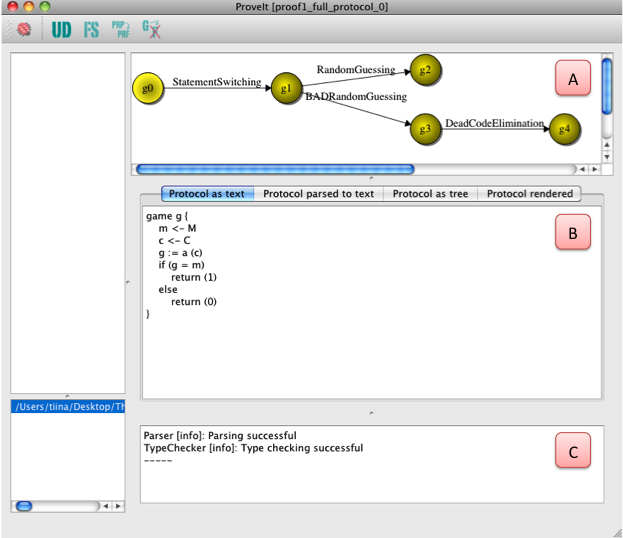
\includegraphics[width=\textwidth]{proveit_screenshot}
% \caption{Screenshot of \proveit.}
% \label{fig:proveit_screenshot}
% \end{center}
% \end{figure}

% Tip: If you add a screenshot then labeling the parts might help make the text more understandable (panel C vs bottom left part), e.g.


% \begin{figure} [htbp]
% \begin{tabular}{c c}
% %
% \begin{minipage}{0.45\textwidth}
% 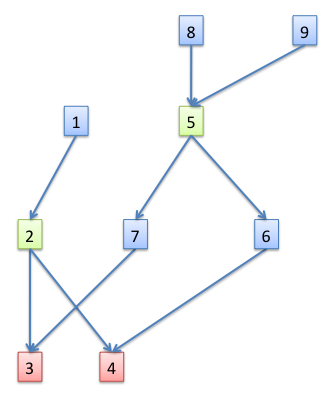
\includegraphics[width=\textwidth]{LCA_2_solutions}
% \end{minipage}
% %
% &
% \begin{minipage}{0.55\textwidth}
% \centering
% \begin{tabular}{ l | l |}
% 	Node & Decendants \\ \hline
%   1 & 2, 3, 4 \\ \hline
%   2 & 3, 4 \\ \hline
%   3 & \\ \hline
%   4 & \\ \hline
%   5 & 3, 4, 6, 7 \\ \hline
%   6 & 4 \\ \hline
%   7 & 3 \\  \hline
%   8 & 3, 4, 5, 6, 7\\ \hline
%   9 & 3, 4, 5, 6, 7\\ \hline
% \end{tabular}
% \end{minipage}
% \end{tabular}
% %
% \caption{Example how to put two figures parallel to each other.}
% \label{fig:LCA_2_solutions}
% \end{figure}


% Example: A screenshot of \proveit can be seen on Figure~\ref{fig:proveit_screenshot}. The user first enters the pseudocode of the initial game in panel B. \proveit also keeps track of all the previous games showing the progress on a graph seen in panel A.

% There are two figures side by side on Figure~\ref{fig:LCA_2_solutions}.



% \clearpage %if newpage doesn't work
% \section{Other Ways to Represent Data}

% \subsection{Tables}

% \begin{table}[h]
% \centering
% \caption{Statements in the \proveit language.}
% \begin{tabular}{| l | l |}
% 	\hline
% 	\bf{Statement} & \bf{Typeset Example} \\
% 	\hline
% 	assignment & $a := 5 + b$ \\
% 	\hline
% 	uniform choice & $m <- M$ \\
% 	\hline
% 	function signature & $f : K \times M -> L$\\
% 	\hline
% \end{tabular}
% \label{tab:statements}
% \end{table}


% \subsection{Lists}

% Numbered list example:
% \begin{enumerate}
% 	\item item one; 
% 	\item item two;
% 	\item item three.
% \end{enumerate} 

% \subsection{Math mode}
% Example:
% \begin{equation}
% a + b = c + d
% \end{equation}
% Aligning:
% \begin{align*}
% 	a &= 5 \\
% 	b + c &= a \\
% 	a -2*3 &= 5/4
% \end{align*}
% Hint: Variables or equations in text are separated with \$ sign, e.g. $a$, $x - y$.

% % \paragraph{Inference Rules}
% % \[ 
% % 	\inference[addition]{x : T & y : T}{x + y : T} 
% % \]
% % Bigger example:
% % \[
% % \inference[assign]{c := a + b & 
% % 	\inference[addG]{a : \typeRat & 
% % 		\inference[var]{b : \typeInt & \typeInt \subseteq \typeRat}{b : \typeRat}
% % 		}{a + b : \typeRat}
% % 	}{c : \typeRat}
% % \]


% \subsection{algorithm2e}

% \begin{algorithm} [!h]
% 	\caption{typeChecking} \label{alg:typeChecking}
% 	\KwIn{Abstract syntax tree}
% 	\KwResult{Type checking result; In addition, type table \typeF{type\_G} for global variables, \typeF{game} for the main game and \typeF{fun} for each $fun \in F$}
% 	\SetKwData{s}{s}
% 	\BlankLine
	
% 	\While{something changed in last cycle}{
% 		\lForEach{global statement \s} {
% 			\parseStatement{\s, \typeF{type\_G}}\;
% 		}
% 		\ForEach{function $fun$} {
% 		\lForEach{statement \s in $fun$} {
% 			\parseStatement{\s, \typeF{fun}}\;
% 		}
% 		}
% 		\lForEach{statement \s in game} {
% 			\parseStatement{\s, \typeF{game}}\;
% 		}
% 	}
% 	%\eIf{error messages were found}{\Return \False\;}{\Return \True\;}
% \end{algorithm}

% \subsection{Pseudocode}

% \begin{figure} [htb]
% \begin{lstlisting}
% expression
%   : NUMBER
%   | VARIABLE
%   | '+' expression
%   | expression '+' expression
%   | expression '*' expression
%   | function_name '(' parameters ')'
%   | '(' expression ')'
% \end{lstlisting}
% \caption{Grammar of arithmetic expressions.}
% \label{fig:parser_exp}
% \end{figure}

% \subsection{Frame Around Information}

% Tip: We can use minipage to create a frame around some important information.
% \begin{figure} [h]
% \frame{
% \begin{minipage}{\textwidth}
% \begin{enumerate}
% 	\item integer division ($\opDiv$) -- only usable between \typeInt types
% 	\item remainder ($\%$) -- only usable between \typeInt types
% \end{enumerate}
% \end{minipage}
% }
% \caption{Arithmetic operations in \proveit revisited.}
% \label{fig:aritmOp_revisit}
% \end{figure}



% \clearpage
% \section{Conclusion}

% \TODO{what did you do?} 
% \TODO{What are the results?}
% \TODO{future work?}

\newpage

% BibTeX bibliography
\bibliographystyle{ieeetr} %plain=[1], alpha=[BGZ09]
\bibliography{unitartucs-thesis}

\addcontentsline{toc}{section}{\refname}


% Use Biblatex if you have problems with Estonian keywords
%\printbibliography %biblatex


% Use alternative local LaTeX bibliography
\begin{comment}
\begin{thebibliography}{9}
\bibitem{proVerif} 
  Bruno Blanchet. 
  Proverif: Cryptographic protocol verifier in the formal model.
  \url{http://www.proverif.ens.fr/}.
  (checked 15.05.2012)
\bibitem{GameB_1} GameB1
\bibitem{GameB_2} GameB2
\bibitem{certicrypt} certicrypt
\bibitem{kamm12} kamm12
\end{thebibliography}
\end{comment}


\newpage
%\appendix
%\section*{\appendixname}
\iflanguage{english}%
  {\section*{Appendix}
  \addcontentsline{toc}{section}{Appendix}
  }%
  {\section*{Lisad}
  \addcontentsline{toc}{section}{Lisad}}


\section*{I. Glossary}
\addcontentsline{toc}{subsection}{I. Glossary}

\newpage

%=== Licence in English
\newcommand{\licencehint}[2]{\\\hspace*{#1}\textsl(#2)\par}
\newcommand\EngLicence{{%
\selectlanguage{english}
\section*{II. Licence}

\addcontentsline{toc}{subsection}{II. Licence}

\subsection*{Non-exclusive licence to reproduce thesis and make thesis public}

I, \textbf{Alice Cooper}, %author's name
  \licencehint{10mm}{author's name}

\begin{enumerate}
\item
herewith grant the University of Tartu a free permit (non-exclusive licence) to
\par
reproduce, for the purpose of preservation, including for adding to the DSpace digital archives until the expiry of the term of copyright,
\par
\textbf{Type Inference for Fourth Order Logic Formulae}, %
  \licencehint{10mm}{title of thesis}
\par
supervised by Axel Rose and May Flower. %supervisor's name
  \licencehint{10mm}{supervisor's name}
\item
I grant the University of Tartu a permit to make the work specified in p. 1 available to the public via the web environment of the University of Tartu, including via the DSpace digital archives, under the Creative Commons licence CC BY NC ND 3.0, which allows, by giving appropriate credit to the author, to reproduce, distribute the work and communicate it to the public, and prohibits the creation of derivative works and any commercial use of the work until the expiry of the term of copyright.
\item
I am aware of the fact that the author retains the rights specified in p. 1 and 2.
\item
I certify that granting the non-exclusive licence does not infringe other persons' intellectual property rights or rights arising from the personal data protection legislation. 
\end{enumerate}

\noindent
Alice Cooper\\ %author's name
\textbf{\textsl{dd/mm/yyyy}}
}}%\newcommand\EngLicence


%=== Licence in Estonian
\newcommand\EstLicence{{%
\selectlanguage{estonian}
\section*{II. Litsents}

\addcontentsline{toc}{subsection}{II. Litsents}

\subsection*{Lihtlitsents lõputöö reprodutseerimiseks ja üldsusele kättesaadavaks tegemiseks}

Mina, \textbf{Alice Cooper}, %author's name
  \licencehint{10mm}{autori nimi}

\begin{enumerate}
\item
annan Tartu Ülikoolile tasuta loa (lihtlitsentsi) minu loodud teose
\par
\textbf{Tüübituletus neljandat järku loogikavalemitele}, %title of thesis
    \licencehint{10mm}{lõputöö pealkiri}
\par
mille juhendaja(d) on Axel Rose ja May Flower, %supervisor's name(s)
  \licencehint{10mm}{juhendaja nimi}
\par
reprodutseerimiseks eesmärgiga seda säilitada, sealhulgas lisada digitaalarhiivi DSpace kuni autoriõiguse kehtivuse lõppemiseni.
\par
\item
Annan Tartu Ülikoolile loa teha punktis 1 nimetatud teos üldsusele kättesaadavaks Tartu Ülikooli veebikeskkonna, sealhulgas digitaalarhiivi DSpace kaudu Creative Commonsi litsentsiga CC BY NC ND 3.0, mis lubab autorile viidates teost reprodutseerida, levitada ja üldsusele suunata ning keelab luua tuletatud teost ja kasutada teost ärieesmärgil, kuni autoriõiguse kehtivuse lõppemiseni.
\item
Olen teadlik, et punktides 1 ja 2 nimetatud õigused jäävad alles ka autorile.
\item
Kinnitan, et lihtlitsentsi andmisega ei riku ma teiste isikute intellektuaalomandi ega isikuandmete kaitse õigusaktidest tulenevaid õigusi. 
\end{enumerate}

\noindent
Alice Cooper\\ %author's name
\textbf{\textsl{pp.kk.aaaa}}
}}%\newcommand\EstLicence


%===Choose the licence in active language
\iflanguage{english}{\EngLicence}{\EstLicence}


\end{document}

